\documentclass[12pt]{article}
\usepackage[utf8]{inputenc}
\usepackage{graphicx}
\usepackage{listings}
\usepackage{amsmath}
\graphicspath{ {./images/} }
\usepackage{amssymb}
\usepackage[htt]{hyphenat}

\usepackage{hyperref}
\hypersetup{
    colorlinks=true,
    linkcolor=blue,
    filecolor=magenta,      
    urlcolor=cyan,
}

\usepackage{xcolor}

\definecolor{codegreen}{rgb}{0,0.6,0}
\definecolor{codegray}{rgb}{0.5,0.5,0.5}
\definecolor{codepurple}{rgb}{0.58,0,0.82}
\definecolor{backcolour}{rgb}{0.95,0.95,0.92}
\definecolor{codeorange}{rgb}{1,0.64,0}

\lstdefinestyle{mystyle}{
    backgroundcolor=\color{backcolour},   
    commentstyle=\color{codegreen},
    keywordstyle=\color{magenta},
    numberstyle=\tiny\color{codeorange},
    stringstyle=\color{codepurple},
    basicstyle=\ttfamily\footnotesize,
    breakatwhitespace=false,         
    breaklines=true,                 
    captionpos=b,                    
    keepspaces=true,                 
    numbers=left,                    
    numbersep=5pt,                  
    showspaces=false,                
    showstringspaces=false,
    showtabs=false,                  
    tabsize=2
}

\lstset{style=mystyle, breaklines=true, postbreak=\mbox{\textcolor{red}{$\hookrightarrow$}\space}}

\title{\vspace{-1cm}Fourier Approximations\\
\large Assignment 4\\
\large EE2703 - Applied Programming Lab}
\author{Abhigyan Chattopadhyay \\
EE19B146}
\date{10th March 2021}
\usepackage[margin=0.75in]{geometry}

\begin{document}
\maketitle
\tableofcontents
\pagebreak
\section{The Problem at Hand}

We want to fit two functions, specifically, $e^x$ and $\cos(\cos(x))$ over the interval $[0,2\pi)$, using the Fourier Series,

$$a_0 + \sum_{n=1}^{\infty}\{a_n\cos(nx)+b_n\sin(nx)\}$$

We will find out these coefficients, $a_n$ and $b_n$ via two different methods, and check how similar they are.

The first method we will use is direct integration using the Fourier series formula,

$$a_0 = \frac{1}{2\pi}\int_{0}^{2\pi}f(x)dx$$
$$a_n = \frac{1}{\pi}\int_{0}^{2\pi}f(x)\cos(x)dx$$
$$b_n = \frac{1}{\pi}\int_{0}^{2\pi}f(x)\sin(x)dx$$

The second method will try to find all the coefficients by solving a matrix equation using the least squares approach we had used last time.

So, without any further ado, let's get started!

\pagebreak
\section{Defining and Plotting the Functions we want to Approximate}

For this program, we will be needing the following libraries:

\begin{enumerate}
    \item \texttt{numpy} (imported as \texttt{np}) for handling matrices and much of the math
    \item \texttt{scipy.integrate.quad} for integrating and finding the the Fourier series coefficients
    \item \texttt{matplotlib.pyplot} (imported as \texttt{plt}) for plotting
\end{enumerate}

\begin{lstlisting}[language=Python]
import numpy as np
from scipy.integrate import quad
import matplotlib.pyplot as plt
import time
\end{lstlisting}

\bigskip
We will use the following \texttt{python} code to define our functions:
\bigskip

\begin{lstlisting}[language=Python]
def expo(x):
    return np.exp(x)

def cc(x):
    return np.cos(np.cos(x))
    
x_vals = np.arange(-2*np.pi,4*np.pi,0.01)
expo_x = expo(x_vals)
cc_x = cc(x_vals)
\end{lstlisting}

\pagebreak
Next, we will plot them using \texttt{matplotlib}

First, for the $e^x$ plot:

\bigskip
\begin{lstlisting}[language=Python]
plt.semilogy(x_vals,expo_x,'r')
plt.grid(True)
plt.ylabel(r'$e^{x}\rightarrow$',fontsize=13)
plt.xlabel(r'x$\rightarrow$',fontsize=13)
plt.title(r'Semi-Log Plot of $e^{x}$',fontsize=16)
plt.savefig("Figure1.png",dpi=1000)
plt.show()
\end{lstlisting}

And the plot generated is shown below:

\begin{center}
    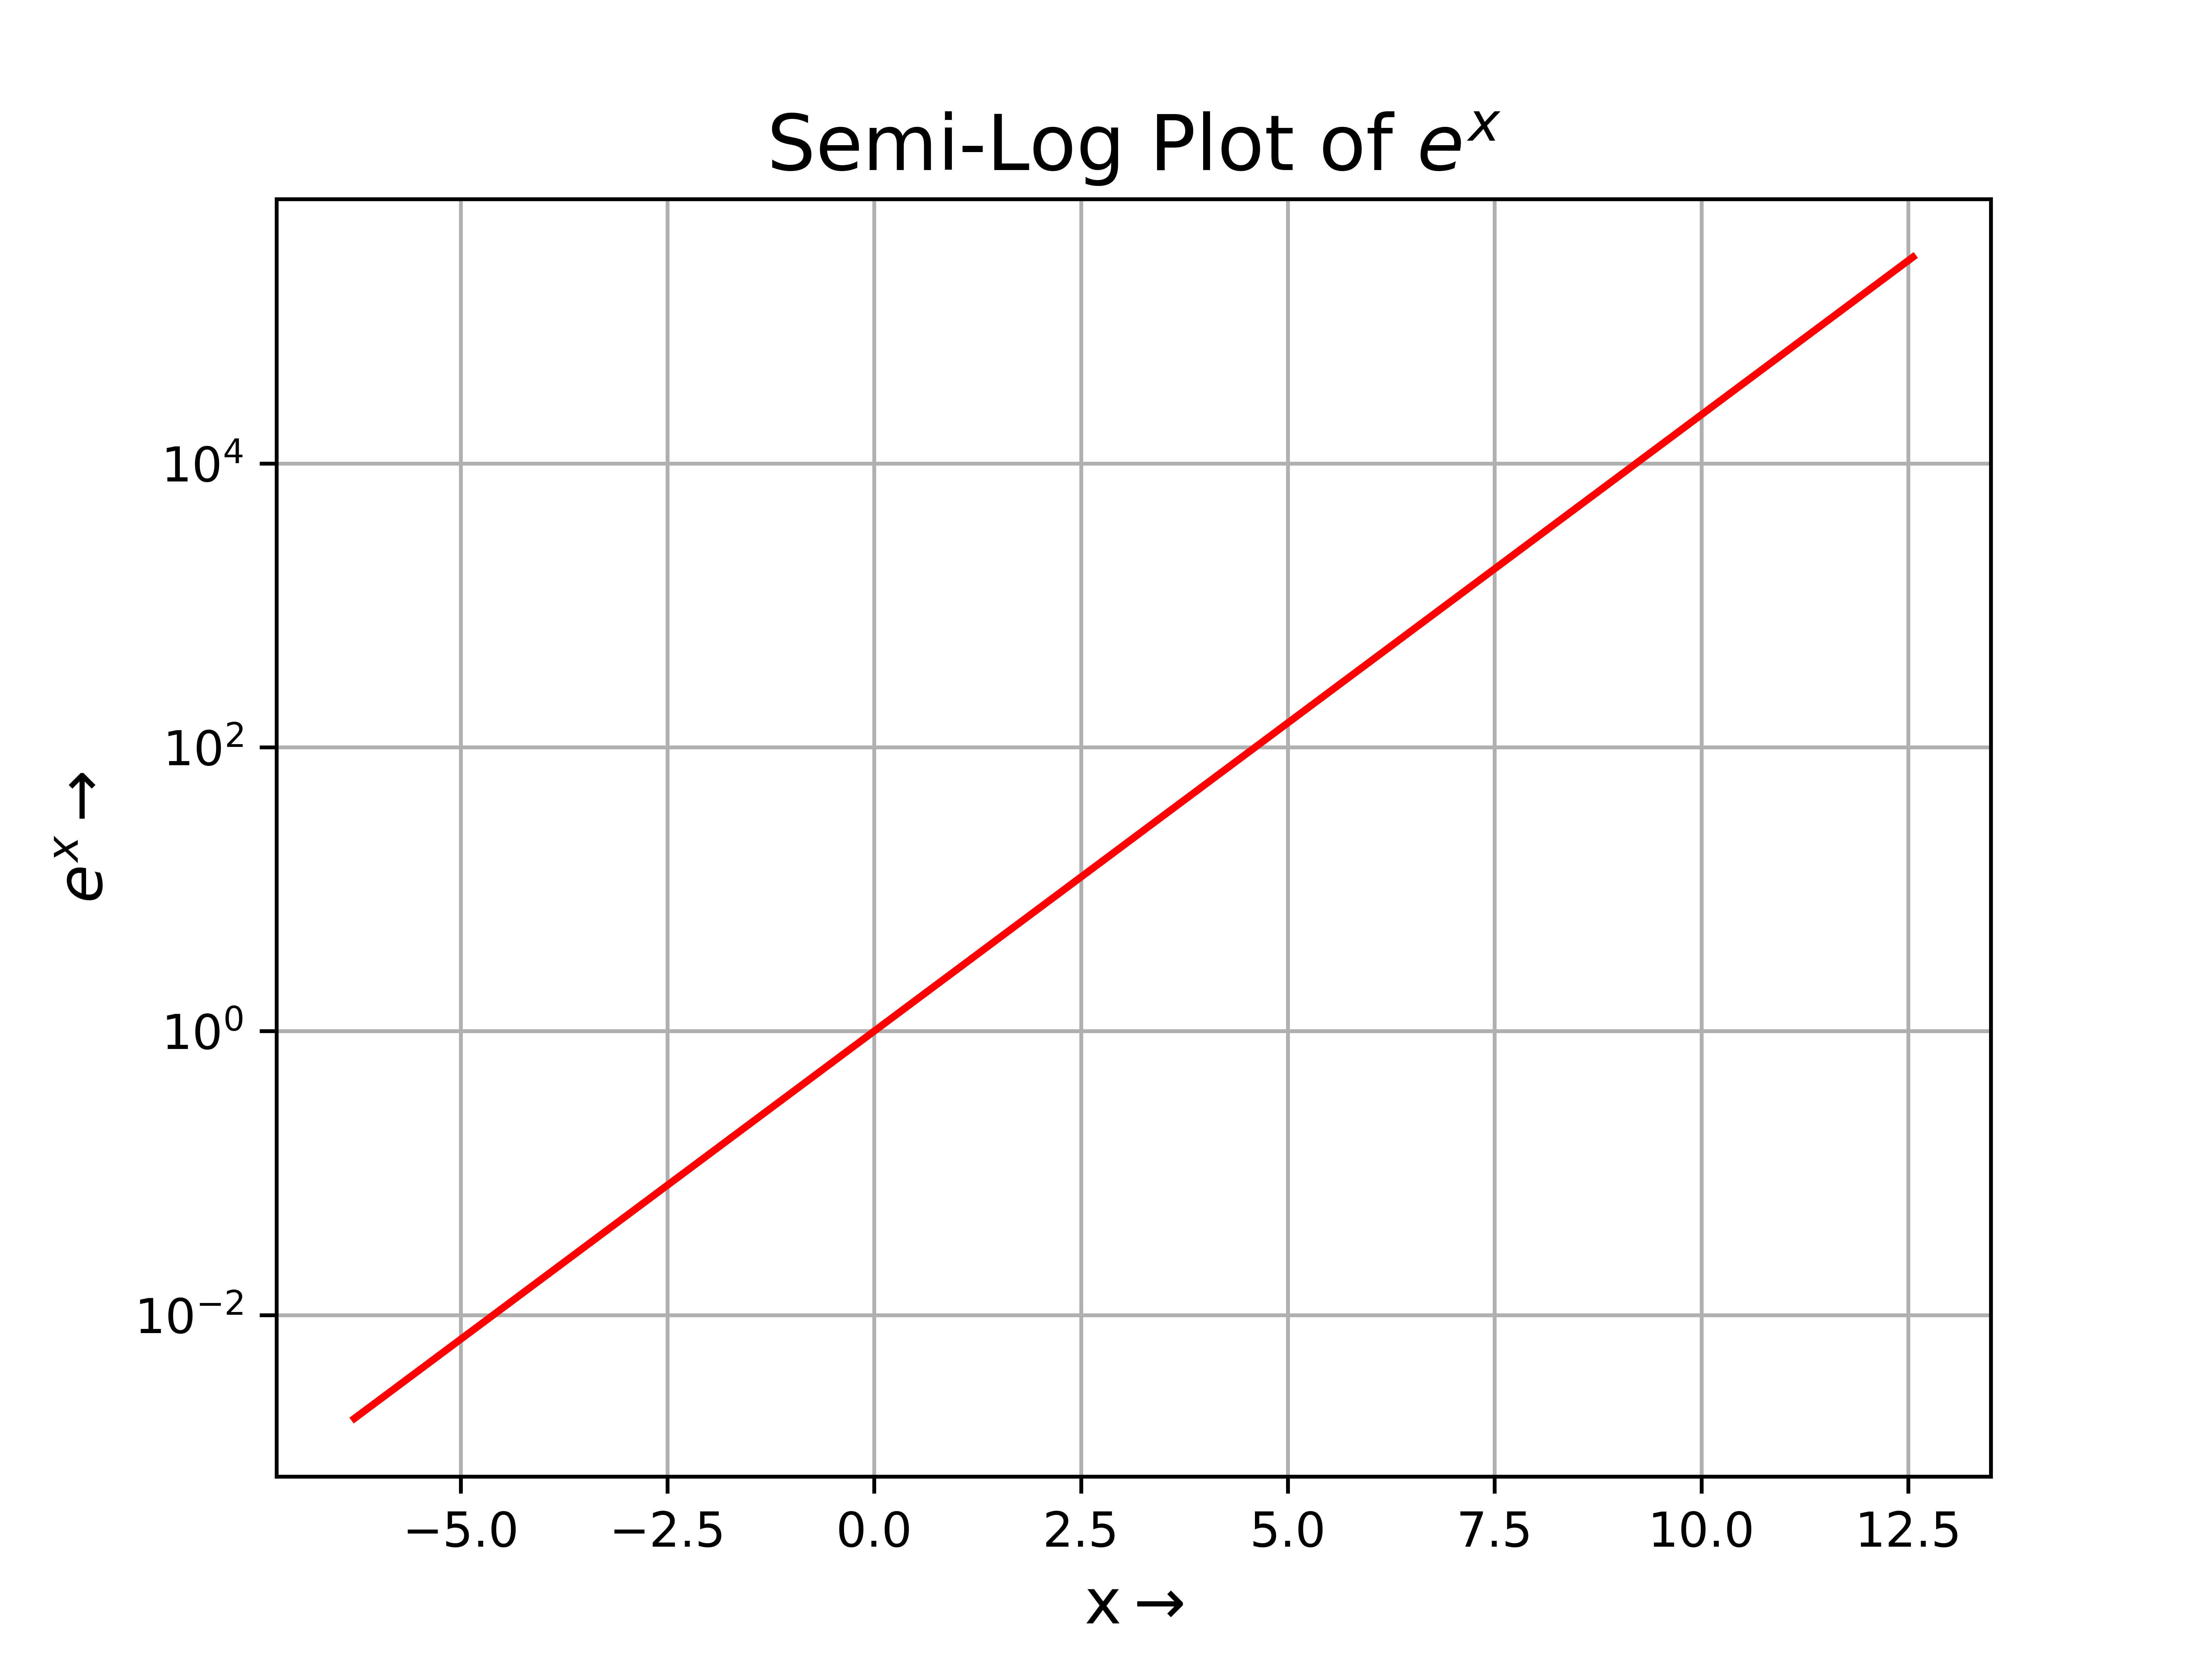
\includegraphics[scale=0.8]{images/Figure1.png}
\end{center}

\bigskip

\pagebreak
Next, we will plot the $\cos(\cos(x))$ graph:
\bigskip
\begin{lstlisting}[language=Python]
plt.plot(x_vals,cc_x,'r')
plt.grid(True)
plt.ylabel(r'$\cos(\cos(x))\rightarrow$',fontsize=13)
plt.xlabel(r'x$\rightarrow$',fontsize=13)
plt.title(r'Plot of $\cos(\cos(x))$',fontsize=16)
plt.savefig("Figure2.png",dpi=1000)
plt.show()
\end{lstlisting}

And the plot generated is shown below:

\begin{center}
    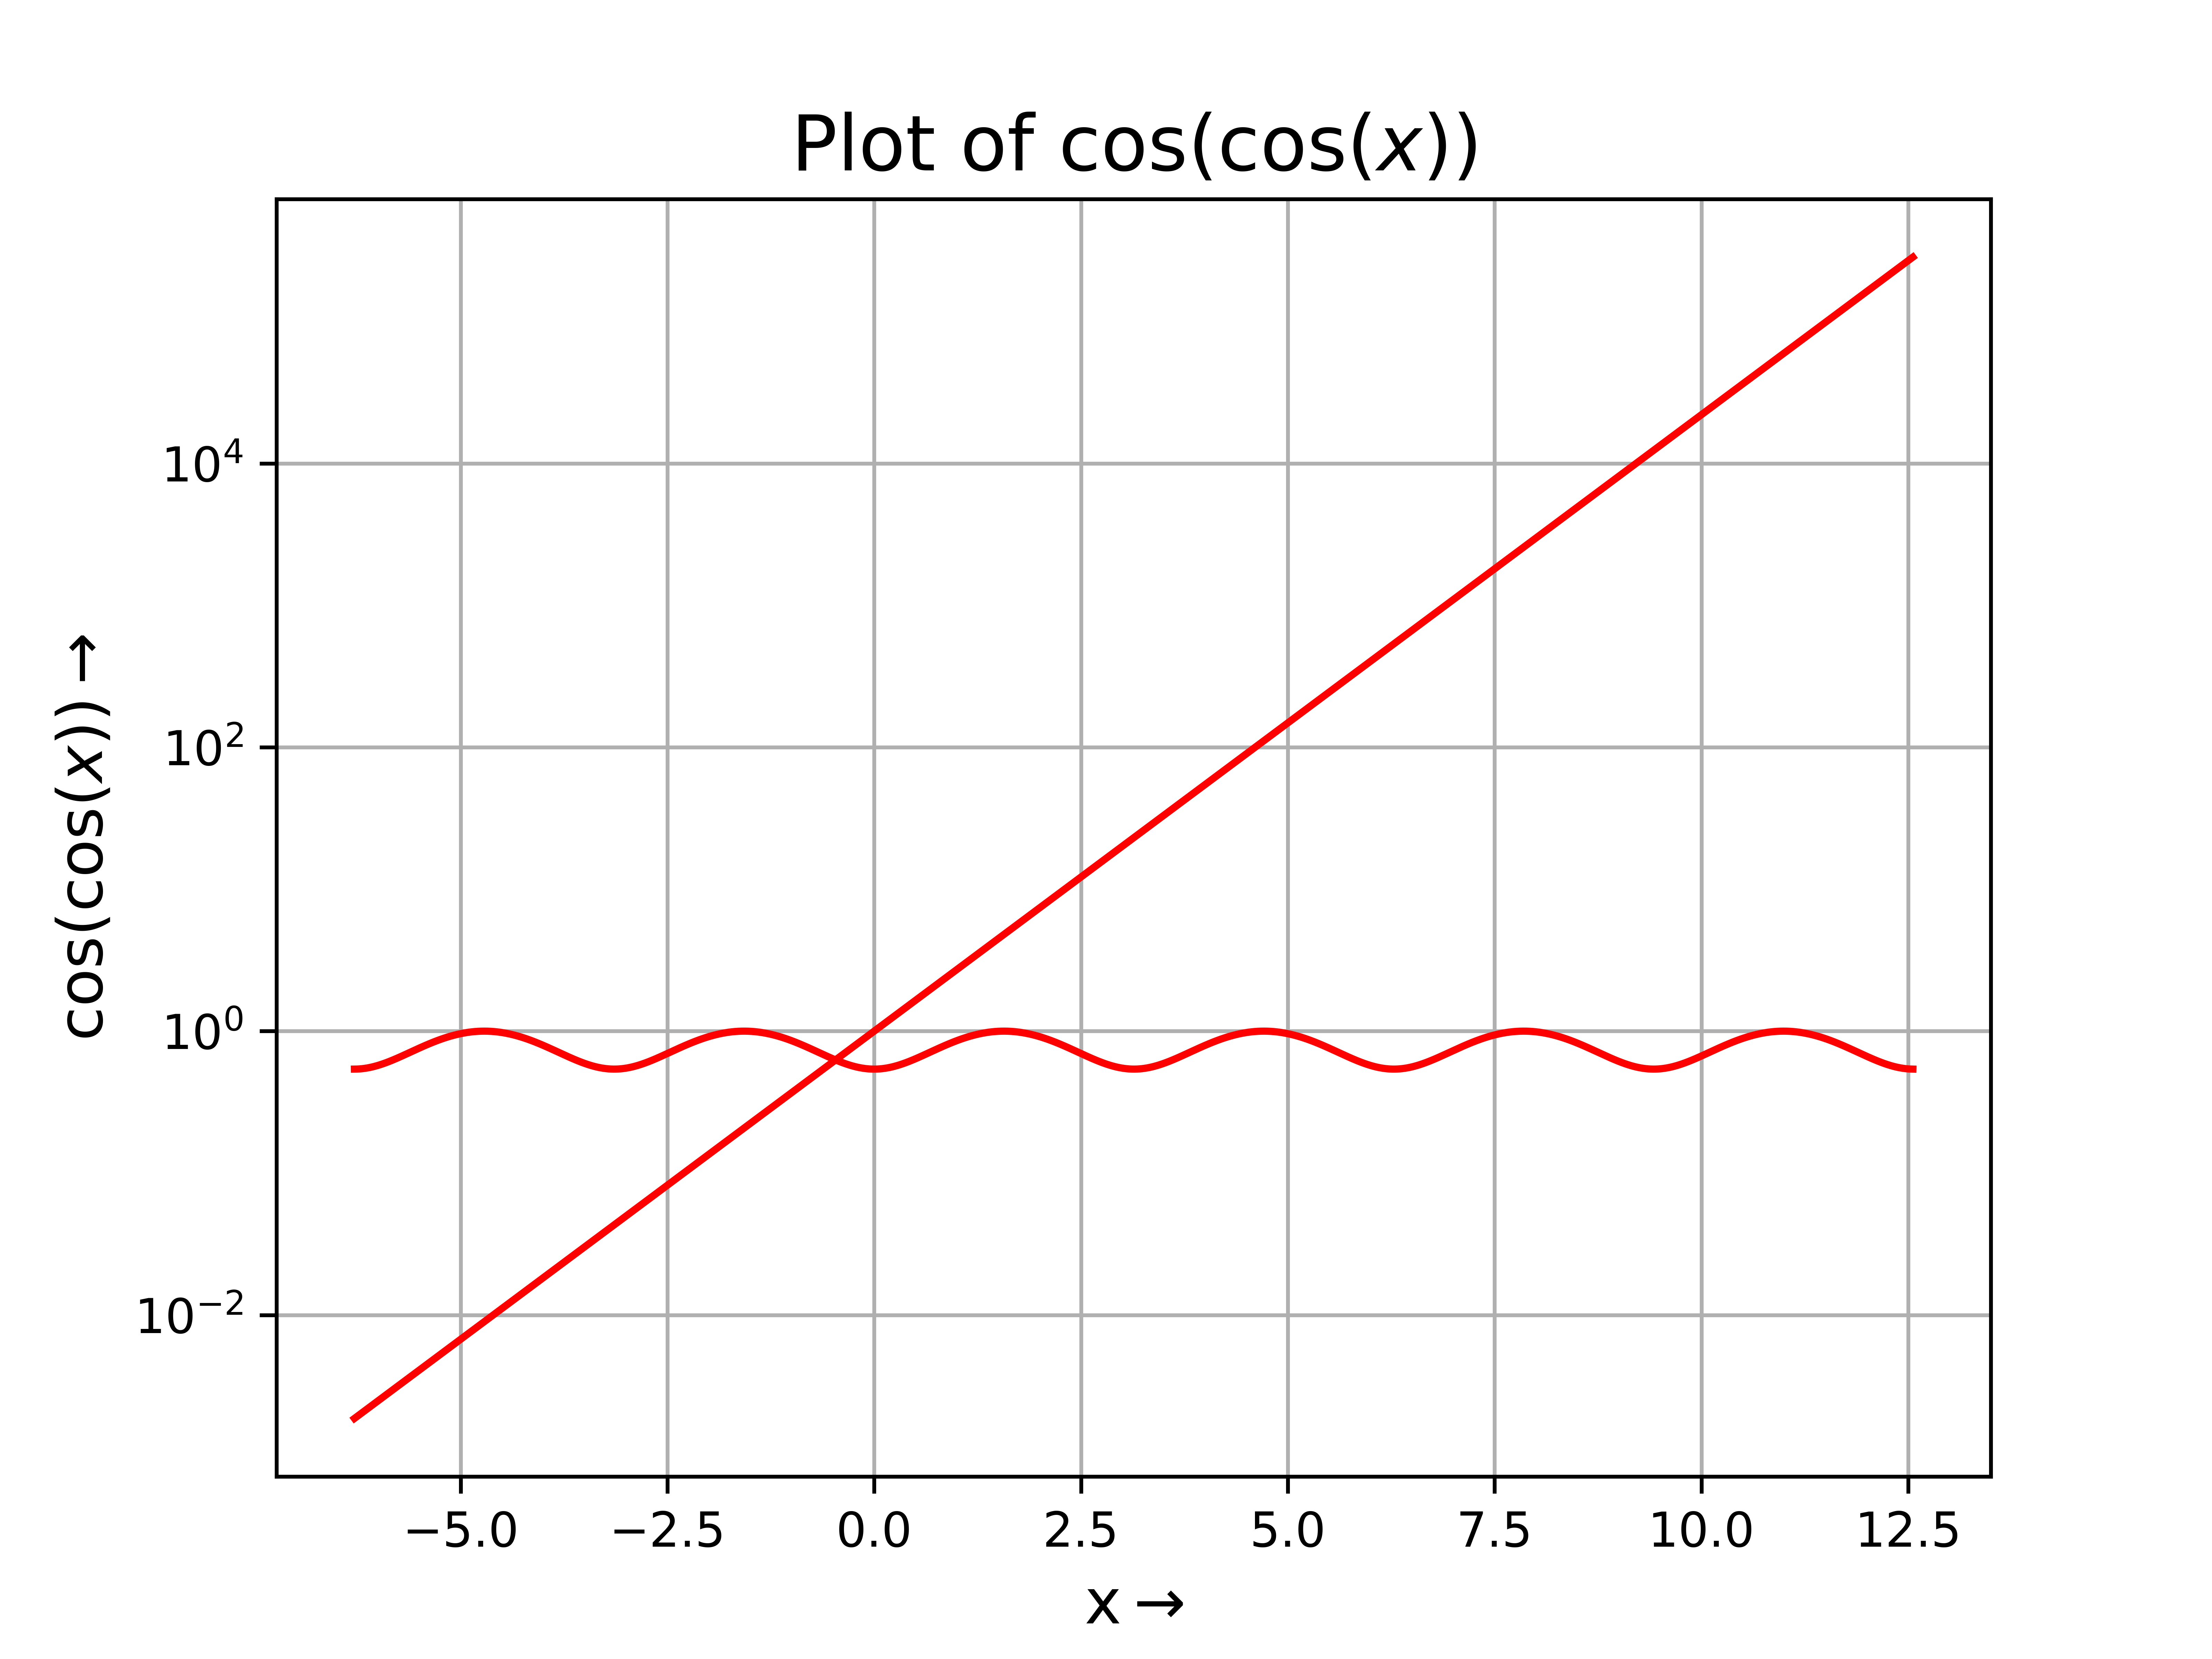
\includegraphics[scale=0.8]{images/Figure2.png}
\end{center}

\pagebreak
\section{Finding the Fourier Series Coefficients by Direct Integration}

We now create a function to integrate a function of our choice and find the first $n$ Fourier coefficients of it:

\begin{lstlisting}[language=Python]
def cfnts_fourier(n,func):
    cfnts = np.zeros(n)
    f = func
    u = lambda x,k: f(x)*np.cos(k*x)
    v = lambda x,k: f(x)*np.sin(k*x)
    cfnts[0]= quad(f,0,2*np.pi)[0]/(2*np.pi)
    for i in range(1,n,2):
        cfnts[i] = quad(u,0,2*np.pi,args=((i+1)/2))[0]/np.pi
    for i in range(2,n,2):
        cfnts[i] = quad(v,0,2*np.pi,args=(i/2))[0]/np.pi
    return cfnts
\end{lstlisting}

\bigskip
\bigskip
Now, we use the function we created to plot Semi-log and Log-Log plots of the Fourier coefficients of the $e^x$ function:

\begin{lstlisting}[language=Python]
t0 = time.time()
expo_cfnts = cfnts_fourier(51,expo)
t1 = time.time()
delTime1 = t1 - t0

plt.semilogy(range(51),abs(expo_cfnts),'ro')
plt.xlabel(r'n$\rightarrow$',fontsize=13)
plt.ylabel(r'Coefficient Magnitudes$\rightarrow$',fontsize=13)
plt.title('Semi-Log Plot of Fourier Series coefficients for $e^{x}$',fontsize=16)
plt.savefig("Figure3.png",dpi=1000)
plt.show()

plt.loglog(range(51),abs(expo_cfnts),'ro')
plt.xlabel(r'n$\rightarrow$',fontsize=13)
plt.ylabel(r'Coefficient Magnitudes$\rightarrow$',fontsize=13)
plt.title('Log-Log Plot of Fourier Series coefficients for $e^{x}$',fontsize=16)
plt.savefig("Figure4.png",dpi=1000)
plt.show()
\end{lstlisting}

\begin{center}
    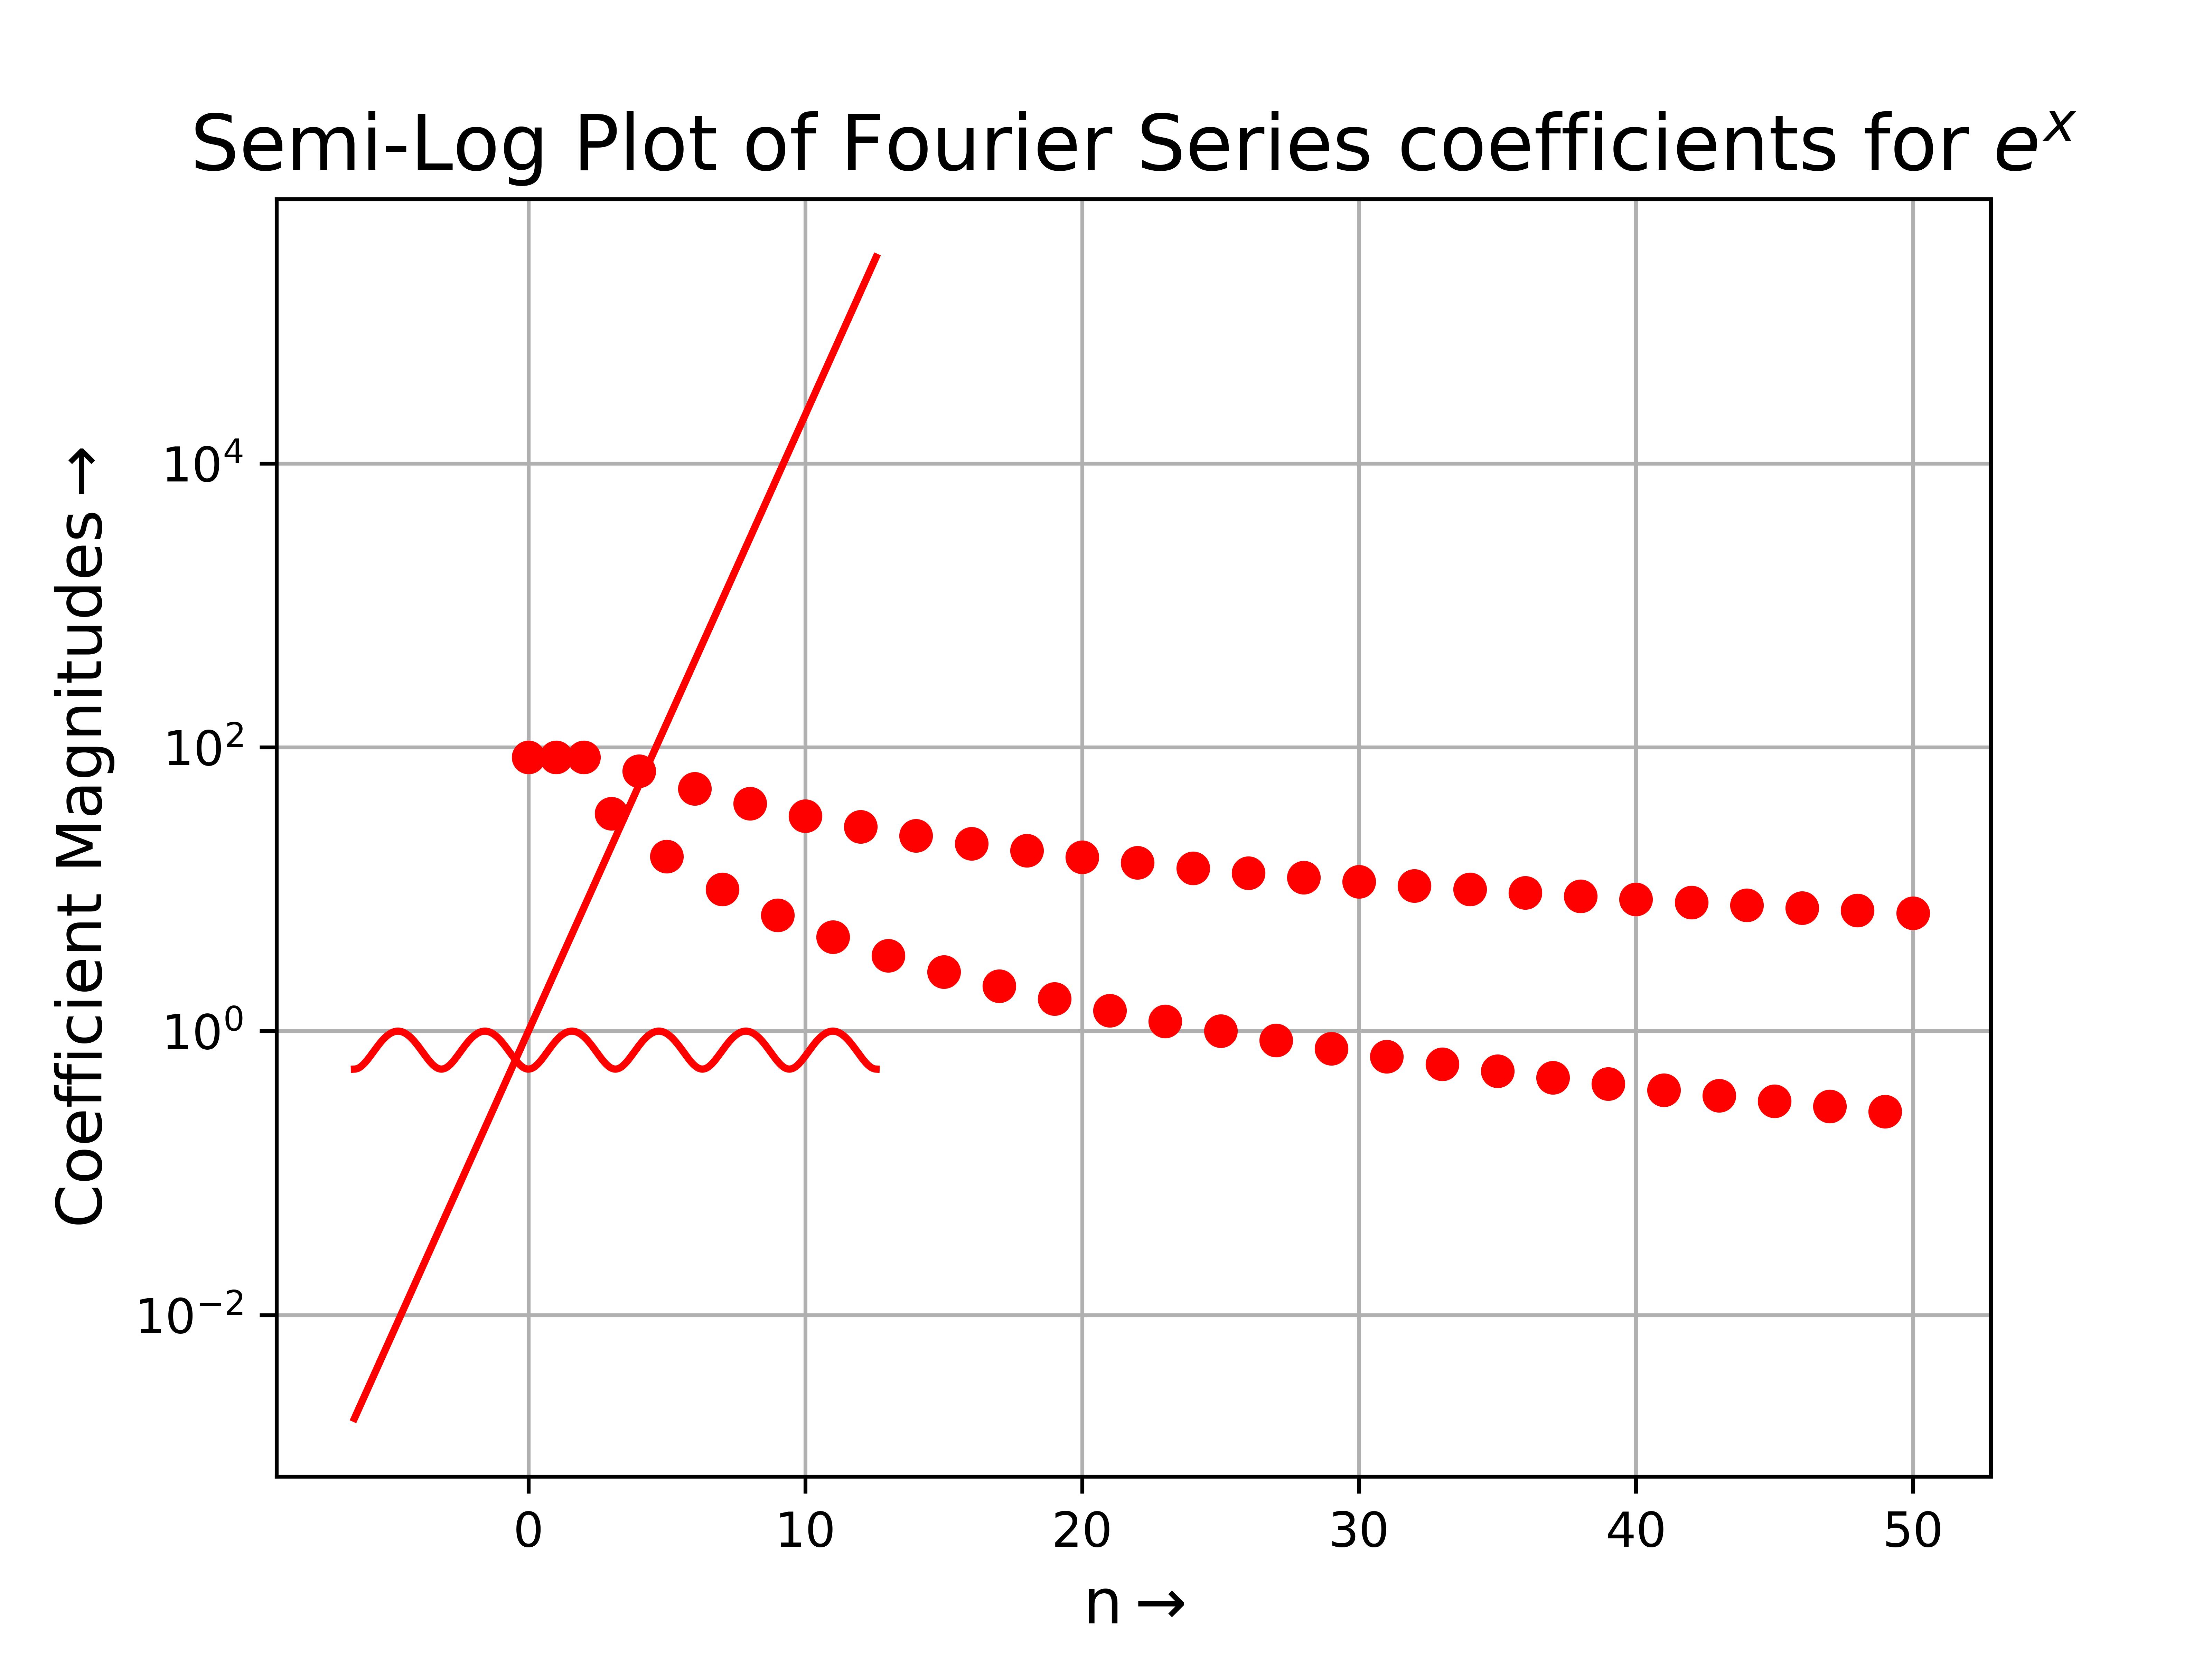
\includegraphics[scale=0.8]{images/Figure3.png}
\end{center}    
    
\begin{center}
    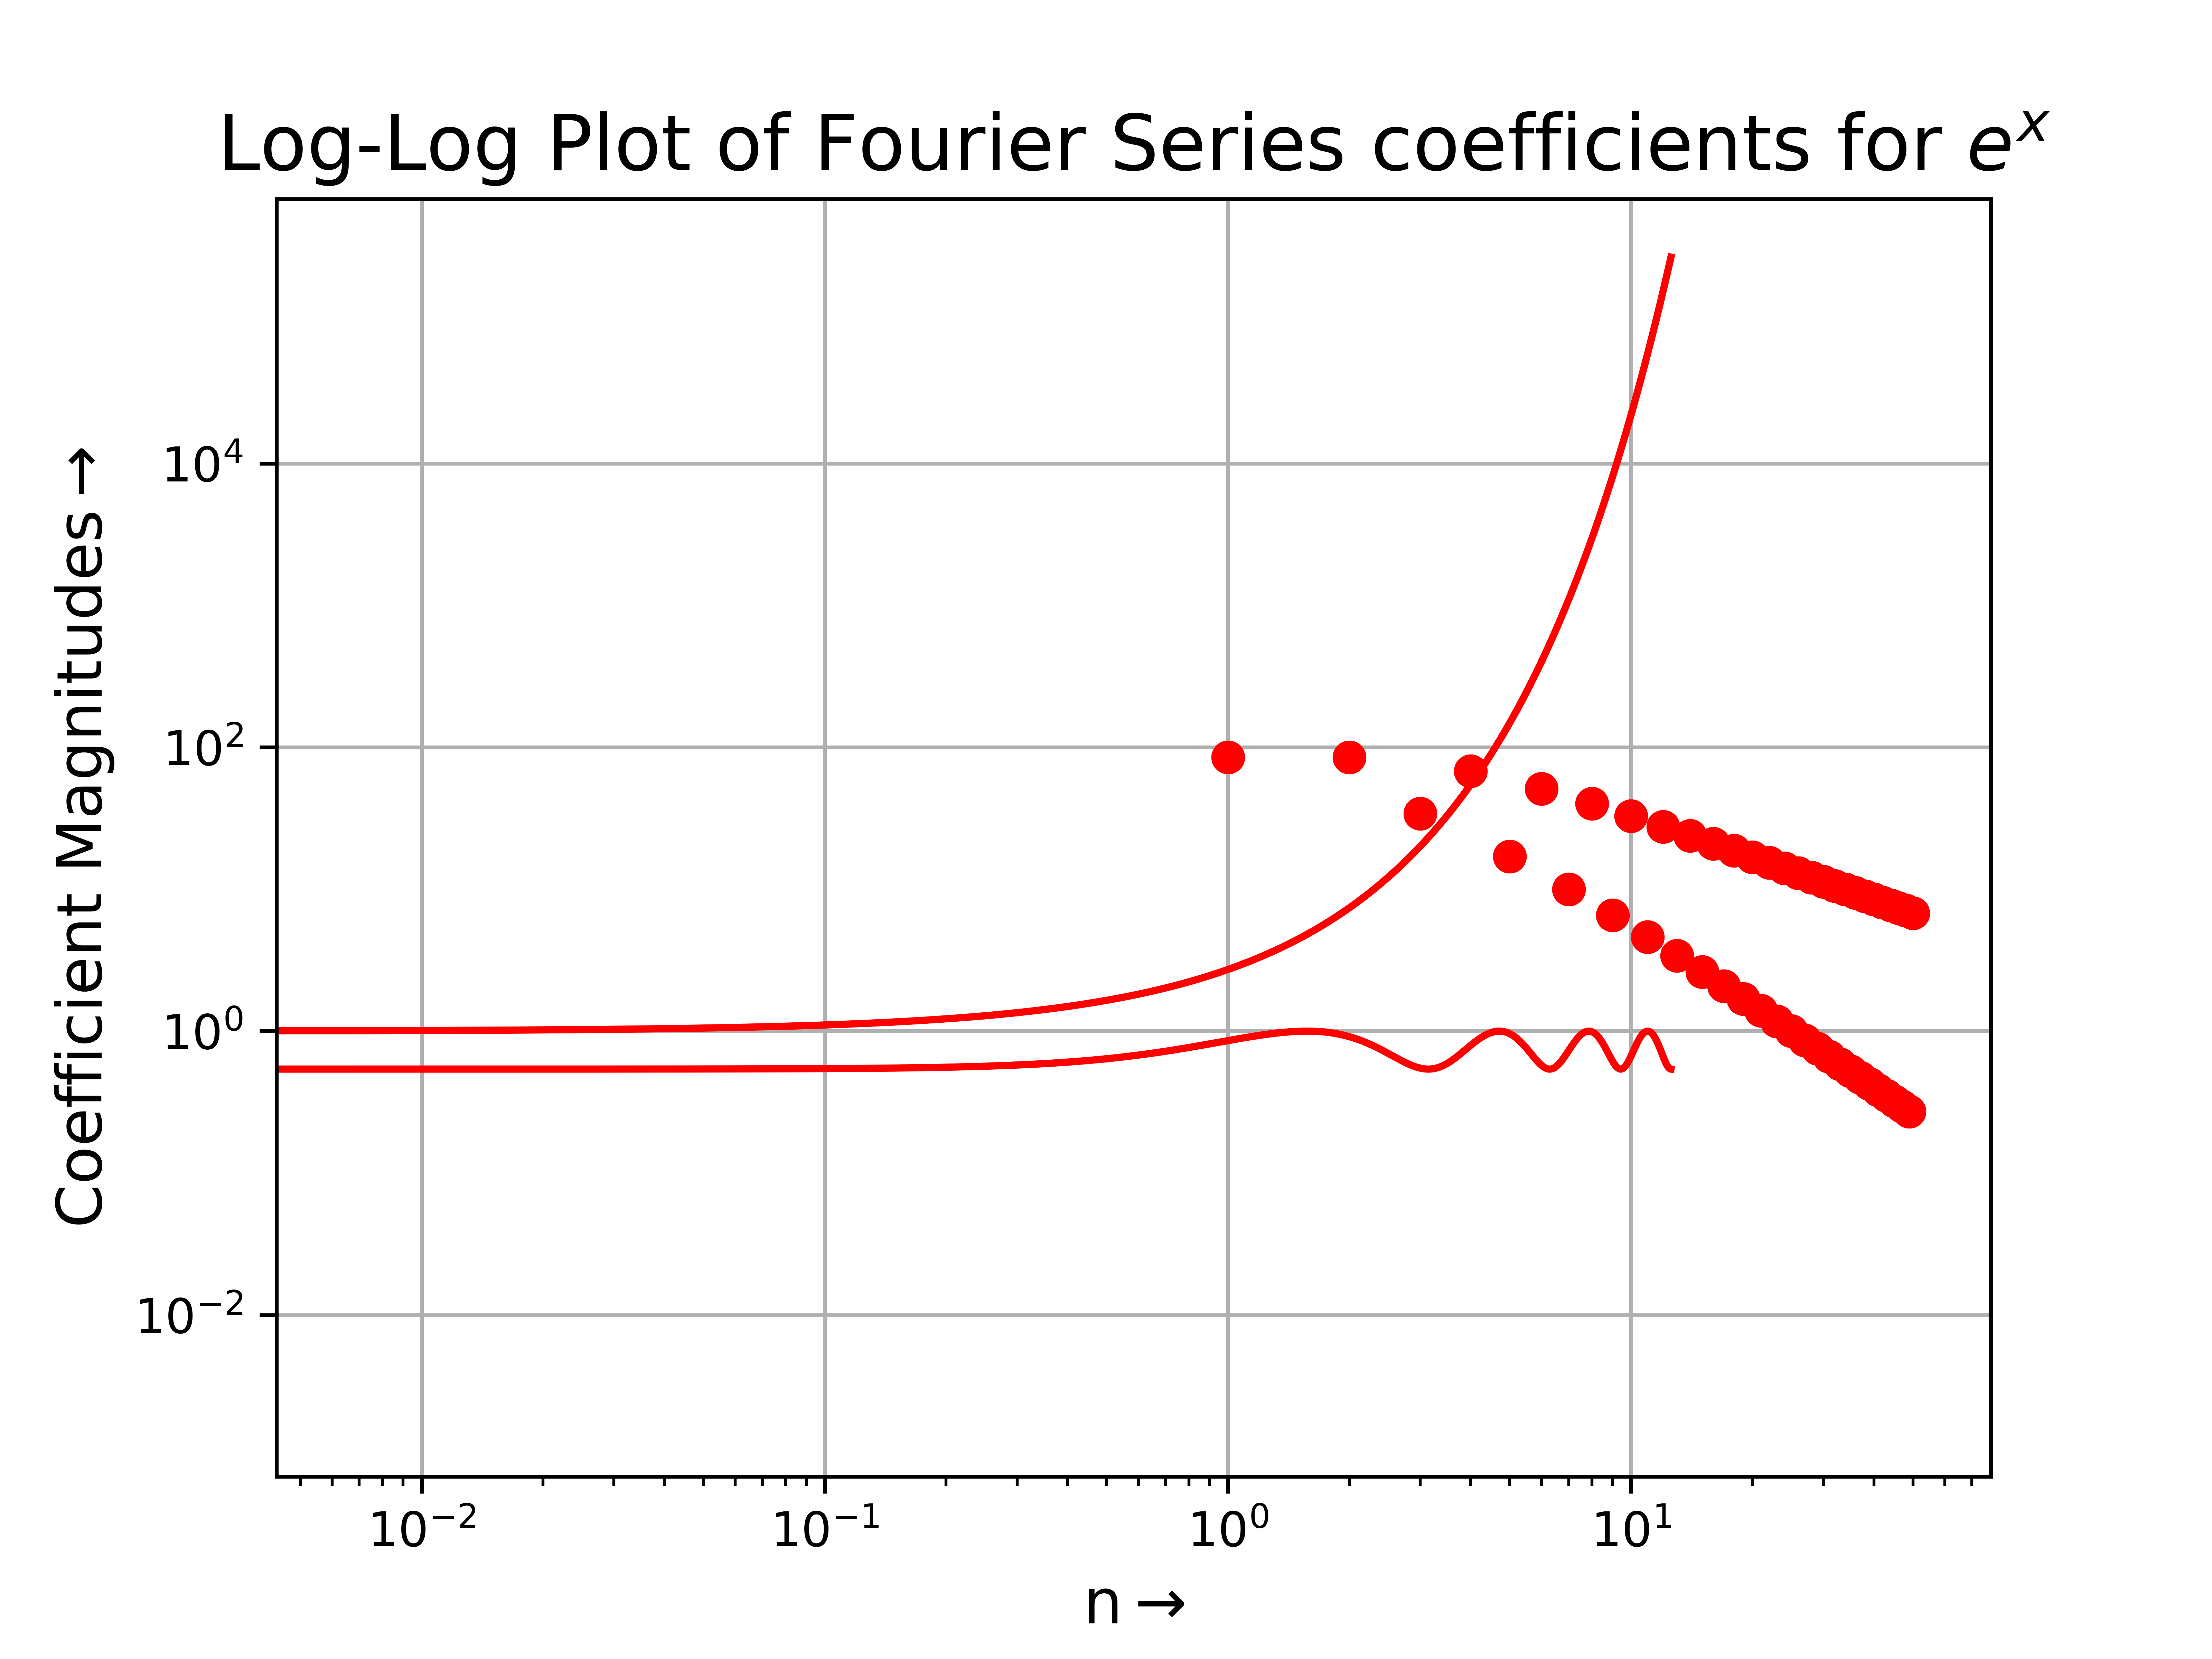
\includegraphics[scale=0.8]{images/Figure4.png}
\end{center}


\pagebreak
Similarly, we plot Semi-log and Log-Log plots of the Fourier coefficients of the $\cos(\cos(x))$ function:

\begin{lstlisting}[language=Python]
t0 = time.time()
cc_cfnts = cfnts_fourier(51,cc)
t1 = time.time()
delTime2 = t1 - t0

plt.semilogy(range(51),abs(cc_cfnts),'ro')
plt.xlabel(r'n$\rightarrow$',fontsize=13)
plt.ylabel(r'Coefficient Magnitudes$\rightarrow$',fontsize=13)
plt.title('Semi-Log Plot of Fourier Series coefficients for $\cos(\cos(x))$',fontsize=16)
plt.savefig("Figure5.png",dpi=1000)
plt.show()

plt.loglog(range(51),abs(cc_cfnts),'ro')
plt.xlabel(r'n$\rightarrow$',fontsize=13)
plt.ylabel(r'Coefficient Magnitudes$\rightarrow$',fontsize=13)
plt.title('Log-Log Plot of Fourier Series coefficients for $\cos(\cos(x))$',fontsize=16)
plt.savefig("Figure6.png",dpi=1000)
plt.show()
\end{lstlisting}

\begin{center}
    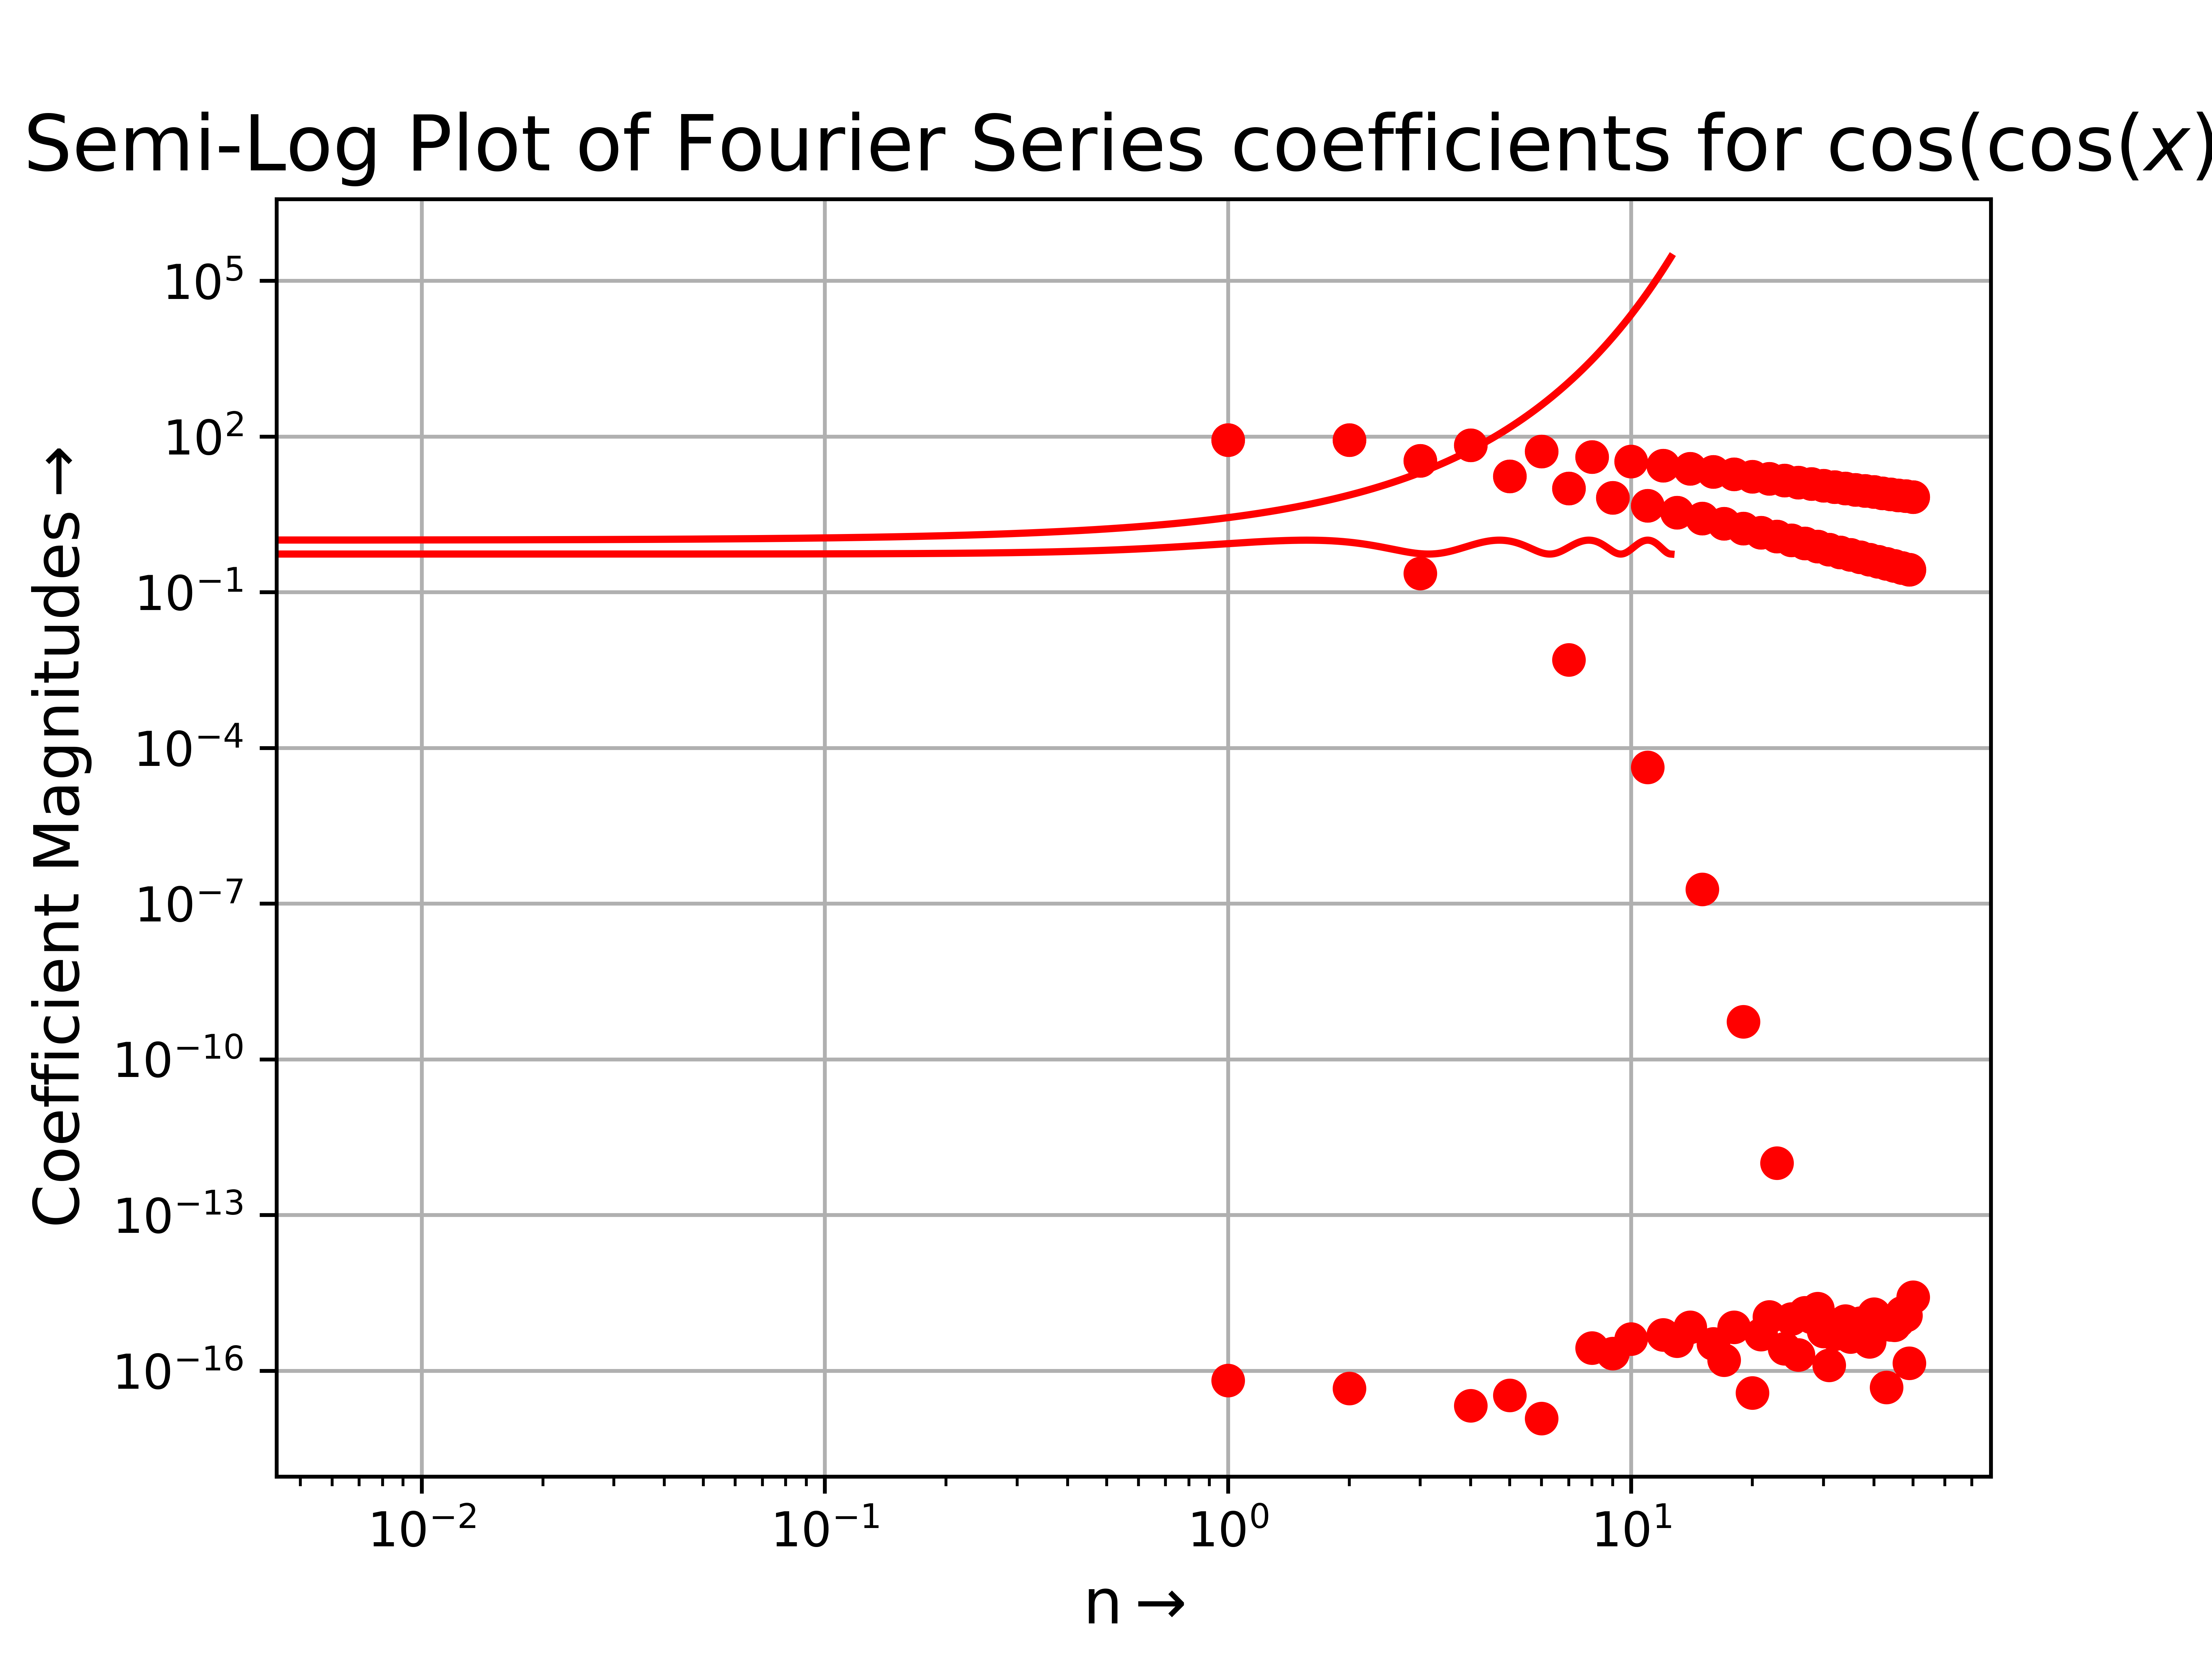
\includegraphics[scale=0.8]{images/Figure5.png}
\end{center}
\begin{center}
    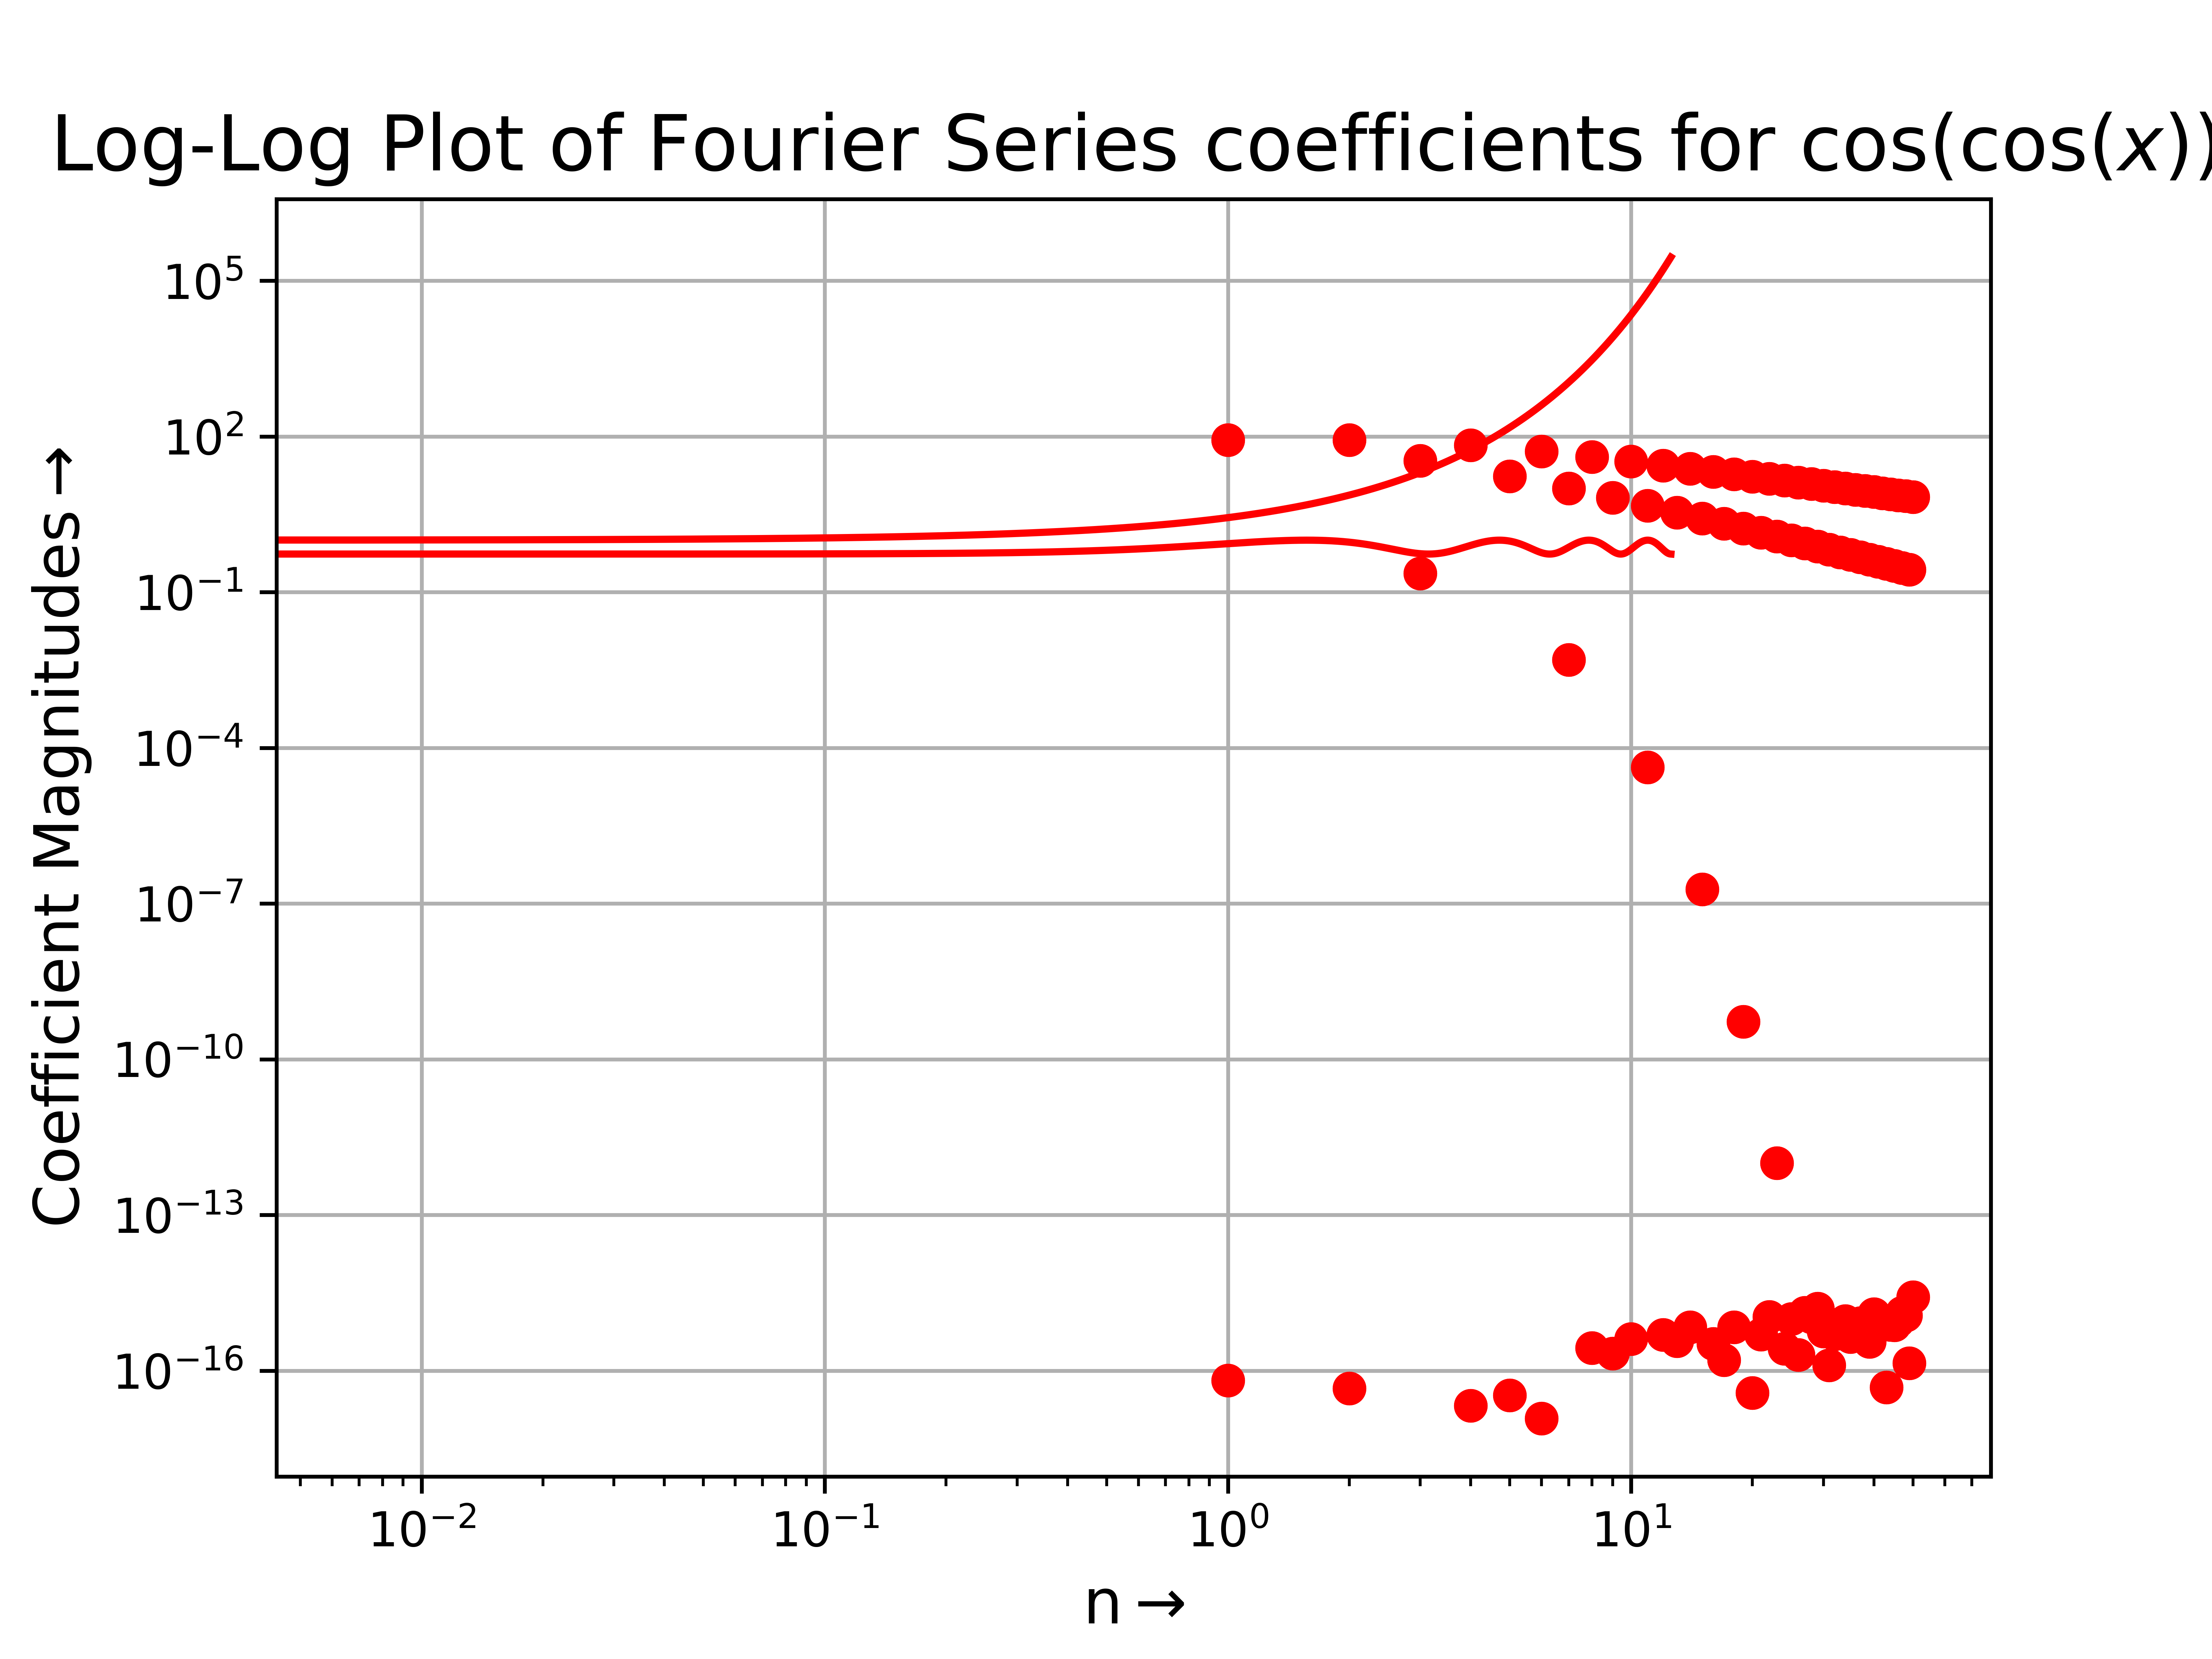
\includegraphics[scale=0.8]{images/Figure6.png}
\end{center}

\subsection{Conclusions Drawn}

\begin{enumerate}
    \item As the function $\cos(\cos(x))$ is even, its $b_n$ coefficients are nearly zero. However, they are not exactly zero due to the numerical limitations of numpy's accuracy.
    \item In the first case, as an exponential has a number of frequencies in it, it has a wide range of frequencies in its Fourier approximation. On the other hand, the second case has only a low frequency of $\frac{1}{\pi}$, and hence has a low contribution from higher sinusoids.
    \item The magnitude of the coefficients of $e^x$ vary as:
    $$|a_n|,|b_n|\propto \frac{1}{1+n^2}$$
    
    Thus, with larger values of $n$, it becomes proportional to $\frac{1}{n^2}$, and hence the log-log plot has a slope of $-2\log n$ and appears to become linear
    
    Similarly, for $\cos(\cos(x))$, the coefficients vary exponentially with $n$, and hence, $\log(y)$ vs $x$ is linear.
\end{enumerate}

\pagebreak
\section{Finding Fourier Series Coefficients using Least Squares}
The Matrix equation is $Ac=b$, where:

$$A = \begin{bmatrix}
1 & \cos(x_1) & \sin(x_1) & \dots & \cos(25x_1) & \sin(25x_1) \\
1 & \cos(x_2) & \sin(x_2) & \dots & \cos(25x_2) & \sin(25x_2) \\
1 & \cos(x_3) & \sin(x_3) & \dots & \cos(25x_3) & \sin(25x_3) \\
\vdots & \vdots & \vdots & \ddots & \vdots & \vdots \\
1 & \cos(x_{399}) & \sin(x_{399}) & \dots & \cos(25x_{399}) & \sin(25x_{399}) \\
1 & \cos(x_{400}) & \sin(x_{400}) & \dots & \cos(25x_{400}) & \sin(25x_{400}) \\
\end{bmatrix}
$$
and 
$$b = \begin{bmatrix}
f(x_1) \\
f(x_2) \\
\vdots \\
f(x_{399}) \\
f(x_{400})
\end{bmatrix}
$$

Now, we will create a function to find the approximate Fourier coefficients using least squares:

\begin{lstlisting}[language=Python]
x = np.linspace(0,2*np.pi,401)
x = x[:-1] # drop last term to have a proper periodic integral
A = np.zeros((400,51)) # an empty matrix A to fill
A[:,0] = 1 # col 1 is all ones
for k in range(1,26):
    A[:,2*k-1] = np.cos(k*x) # cos(kx) column
    A[:,2*k] = np.sin(k*x) # sin(kx) column

def cfnts_lstsq(func,A,x):
    b = func(x) # func takes a vector input and returns a vector output
    cfnts=np.linalg.lstsq(A,b,rcond=None)[0]
    # the '[0]' is to pull out the best fit vector. lstsq returns a list.
    return cfnts
\end{lstlisting}
\pagebreak

Now, we will plot the exponential function's Fourier Coefficients obtained by Least Squares:

\begin{lstlisting}[language=Python]
t0 = time.time()
expo_lstsq = cfnts_lstsq(expo,A,x)
t1 = time.time()
delTime3 = t1 - t0

plt.semilogy(range(51),abs(expo_lstsq),'go')
plt.xlabel(r'n$\rightarrow$',fontsize=13)
plt.ylabel(r'Coefficient Magnitudes$\rightarrow$',fontsize=13)
plt.title('Semi-Log Plot of Fourier Series coefficients for $e^{x}$',fontsize=16)
plt.savefig("Figure7.png",dpi=1000)
plt.show()

plt.loglog(range(51),abs(expo_lstsq),'go')
plt.xlabel(r'n$\rightarrow$',fontsize=13)
plt.ylabel(r'Coefficient Magnitudes$\rightarrow$',fontsize=13)
plt.title('Log-Log Plot of Fourier Series coefficients for $e^{x}$',fontsize=16)
plt.savefig("Figure8.png",dpi=1000)
plt.show()
\end{lstlisting}

\begin{center}
    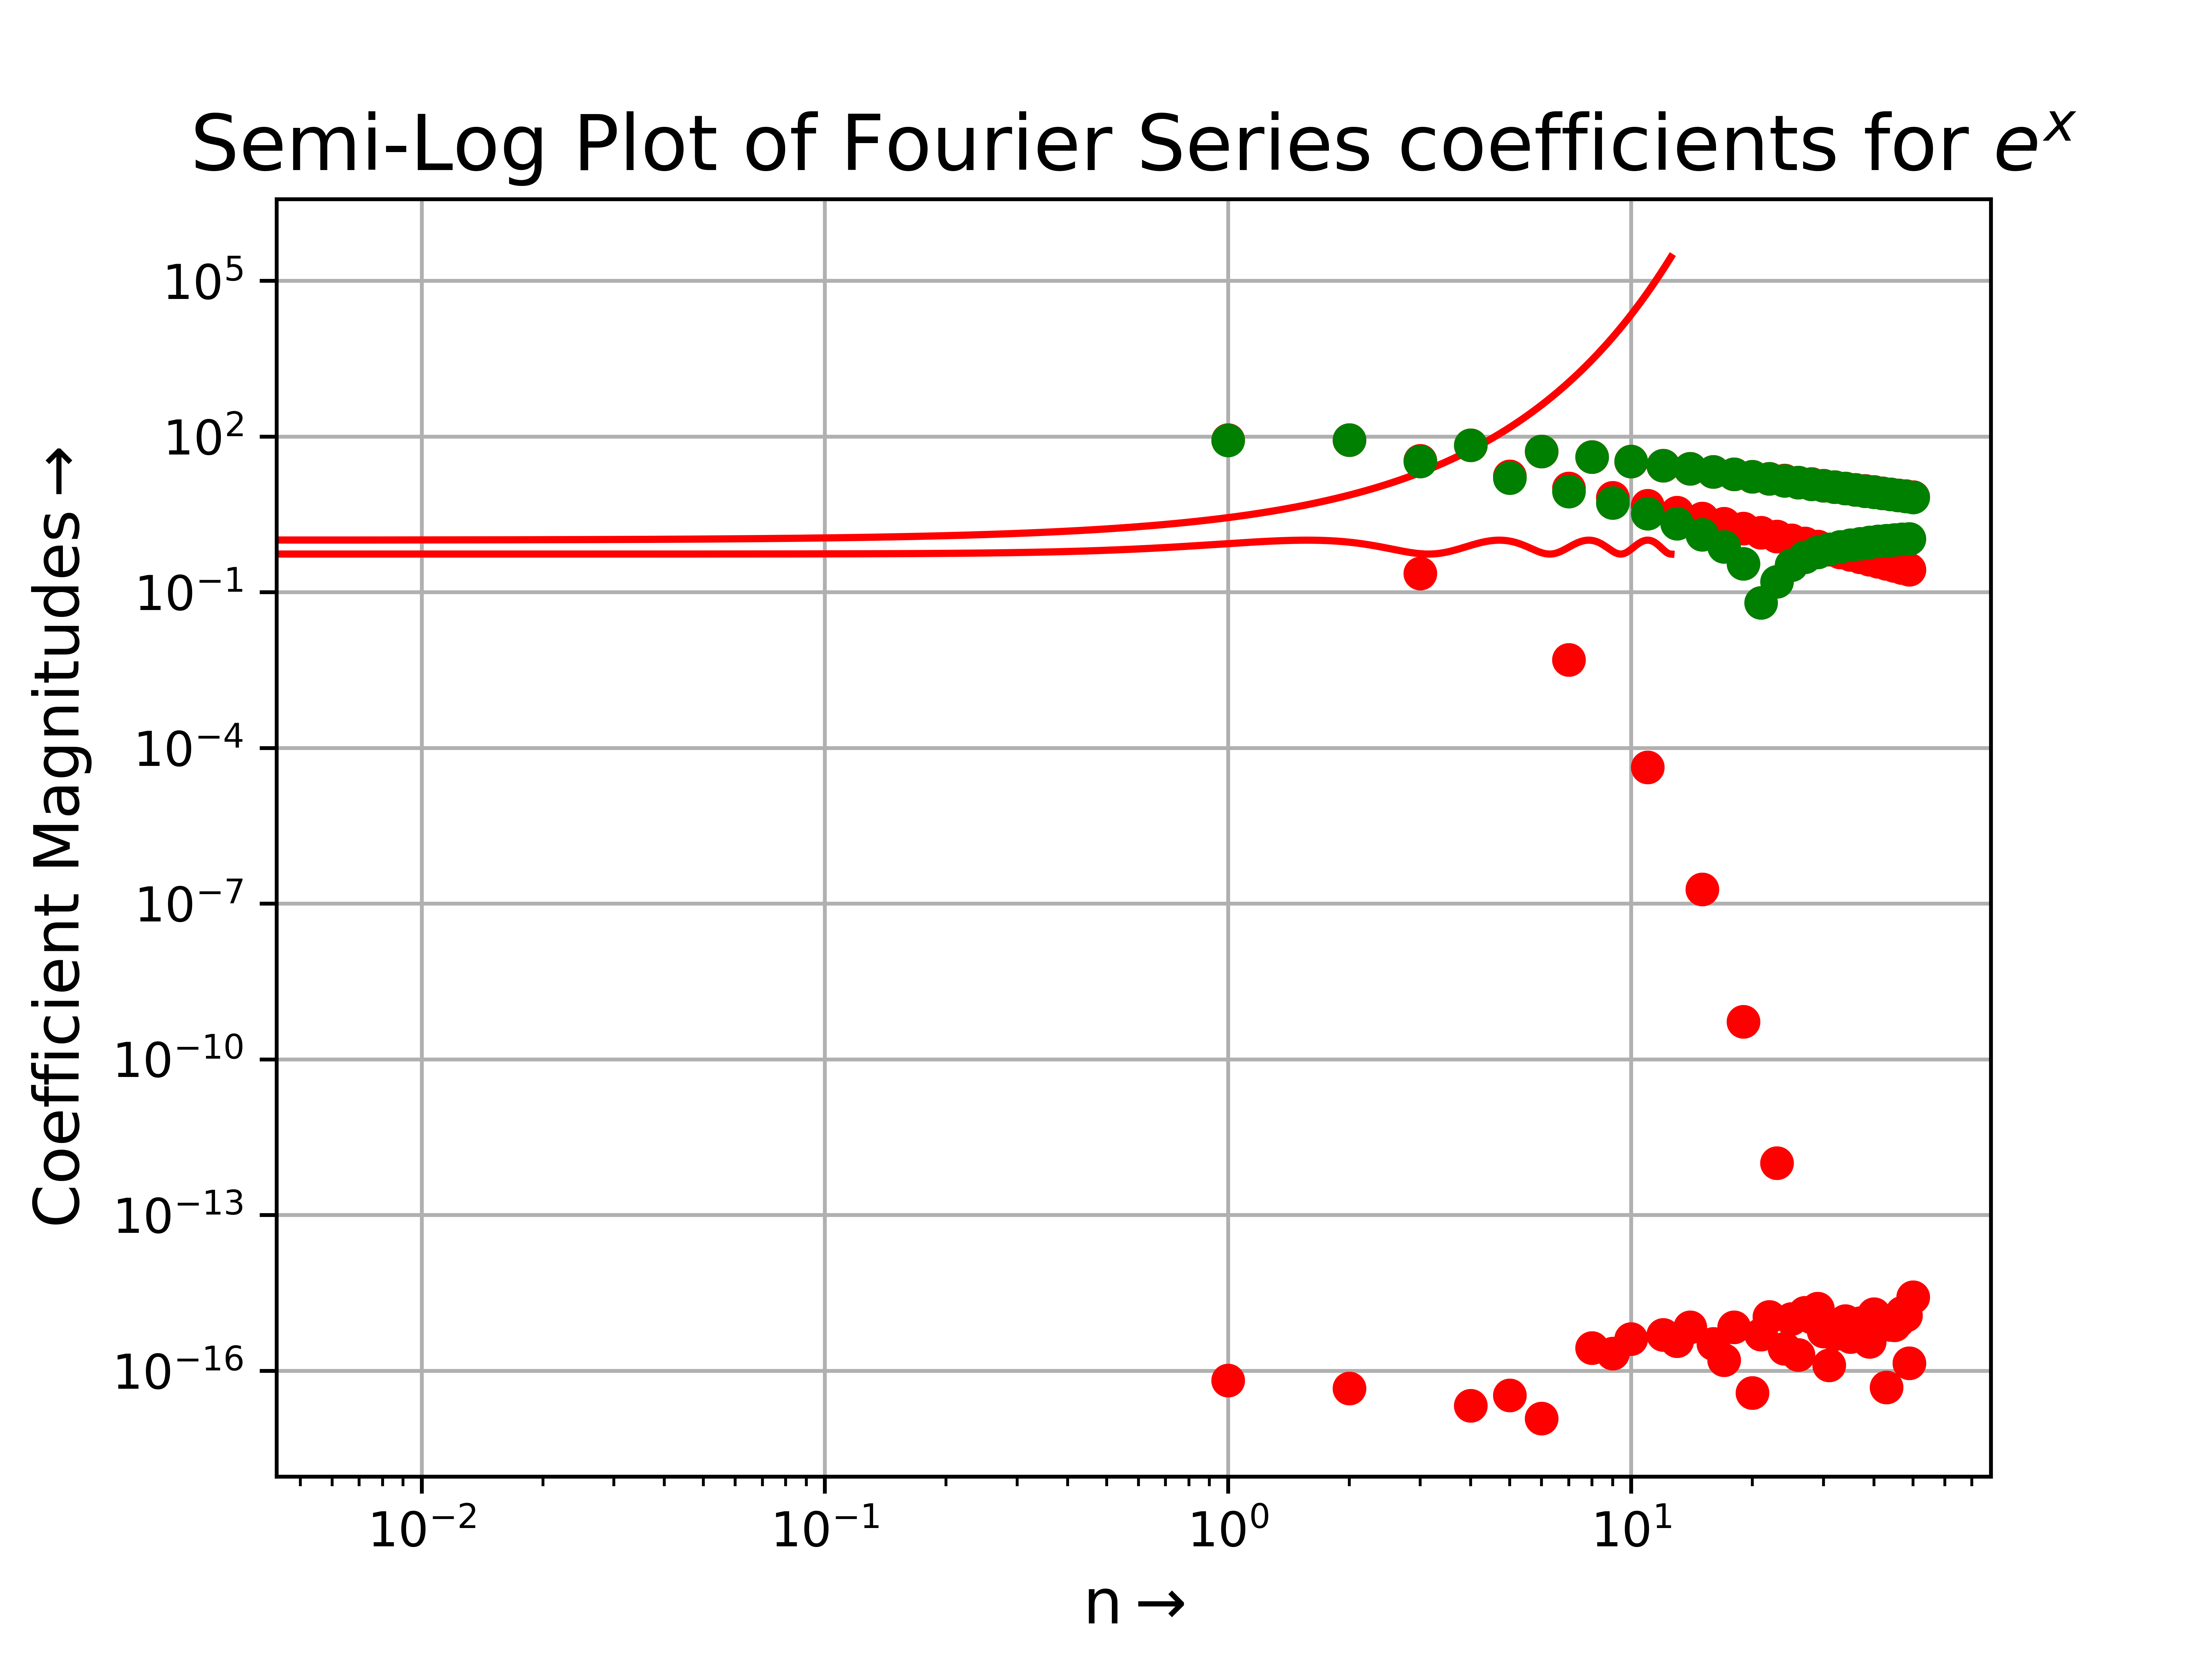
\includegraphics[scale=0.8]{images/Figure7.png}
\end{center}
\begin{center}
    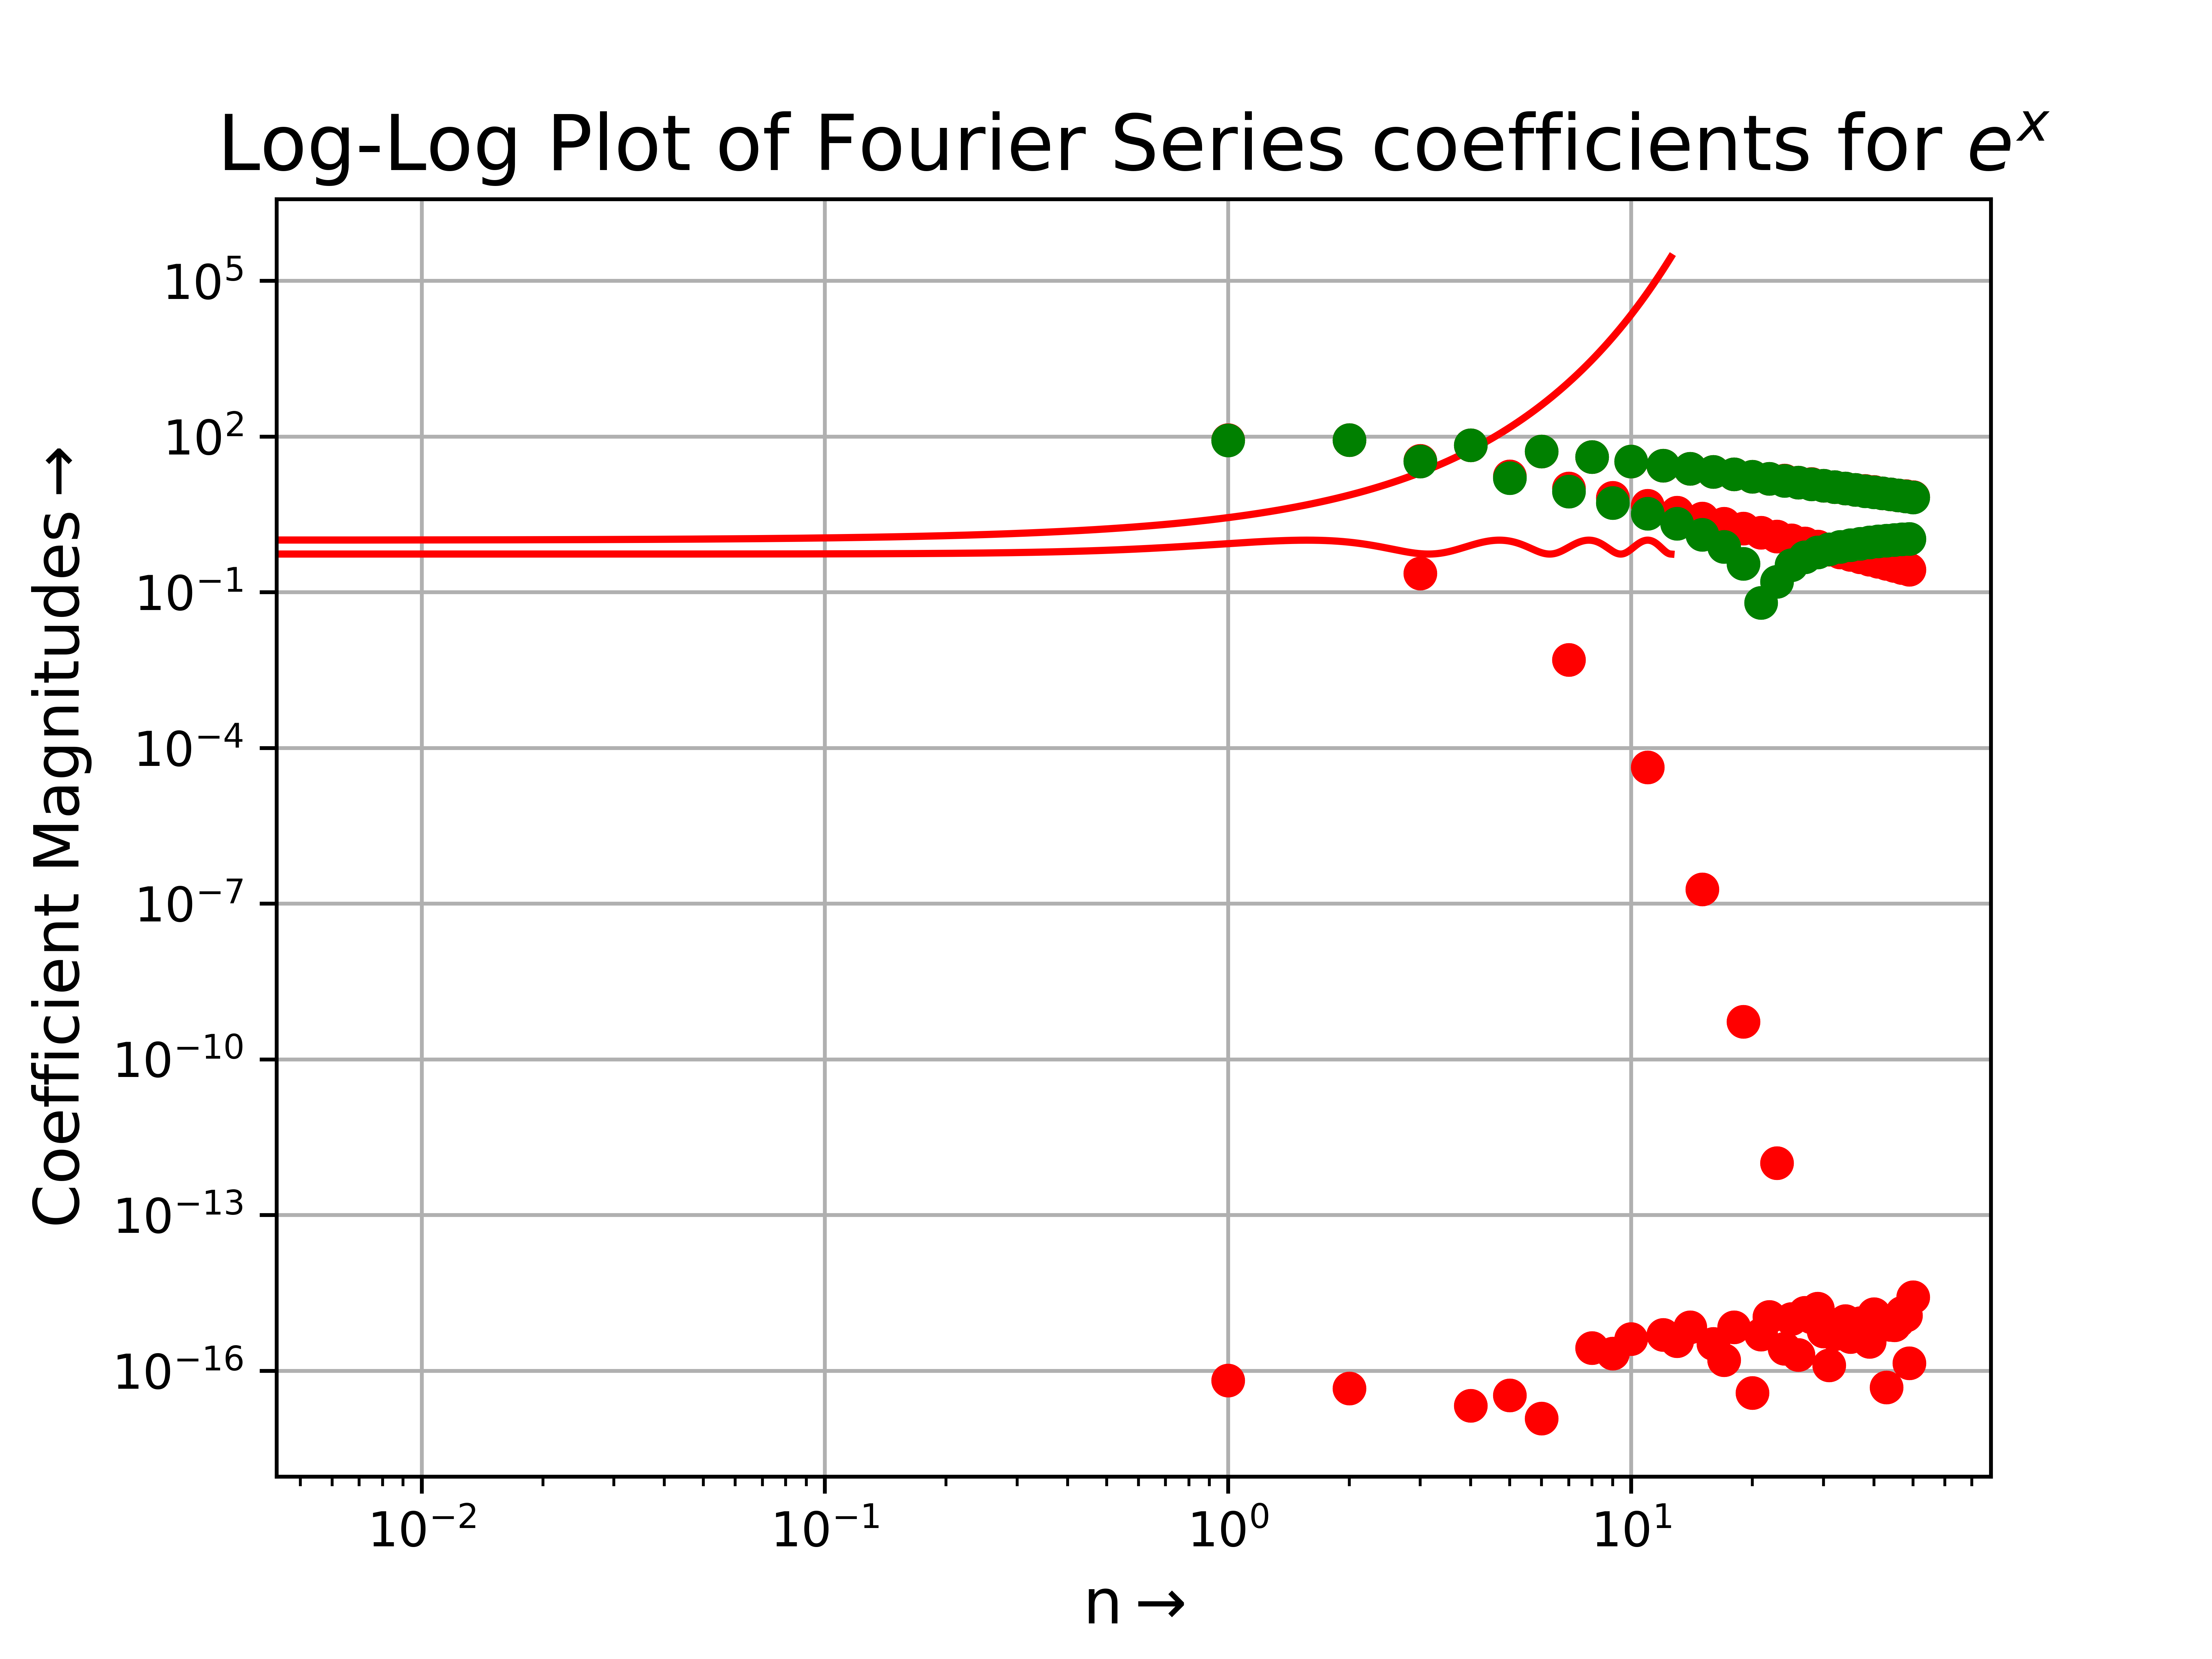
\includegraphics[scale=0.8]{images/Figure8.png}
\end{center}
\pagebreak

Similarly, now we will plot the $\cos(\cos(x))$ function's Fourier Coefficients obtained by Least Squares:

\begin{lstlisting}[language=Python]
t0 = time.time()
cc_lstsq = cfnts_lstsq(cc,A,x)
t1 = time.time()
delTime4 = t1 - t0

plt.semilogy(range(51),abs(cc_lstsq),'go')
plt.xlabel(r'n$\rightarrow$',fontsize=13)
plt.ylabel(r'Coefficient Magnitudes$\rightarrow$',fontsize=13)
plt.title('Semi-Log Plot of Fourier Series coefficients for $\cos(\cos(x))$',fontsize=16)
plt.savefig("Figure9.png",dpi=1000)
plt.show()

plt.loglog(range(51),abs(cc_lstsq),'go')
plt.xlabel(r'n$\rightarrow$',fontsize=13)
plt.ylabel(r'Coefficient Magnitudes$\rightarrow$',fontsize=13)
plt.title('Log-Log Plot of Fourier Series coefficients for $\cos(\cos(x))$',fontsize=16)
plt.savefig("Figure10.png",dpi=1000)
plt.show()
\end{lstlisting}

\begin{center}
    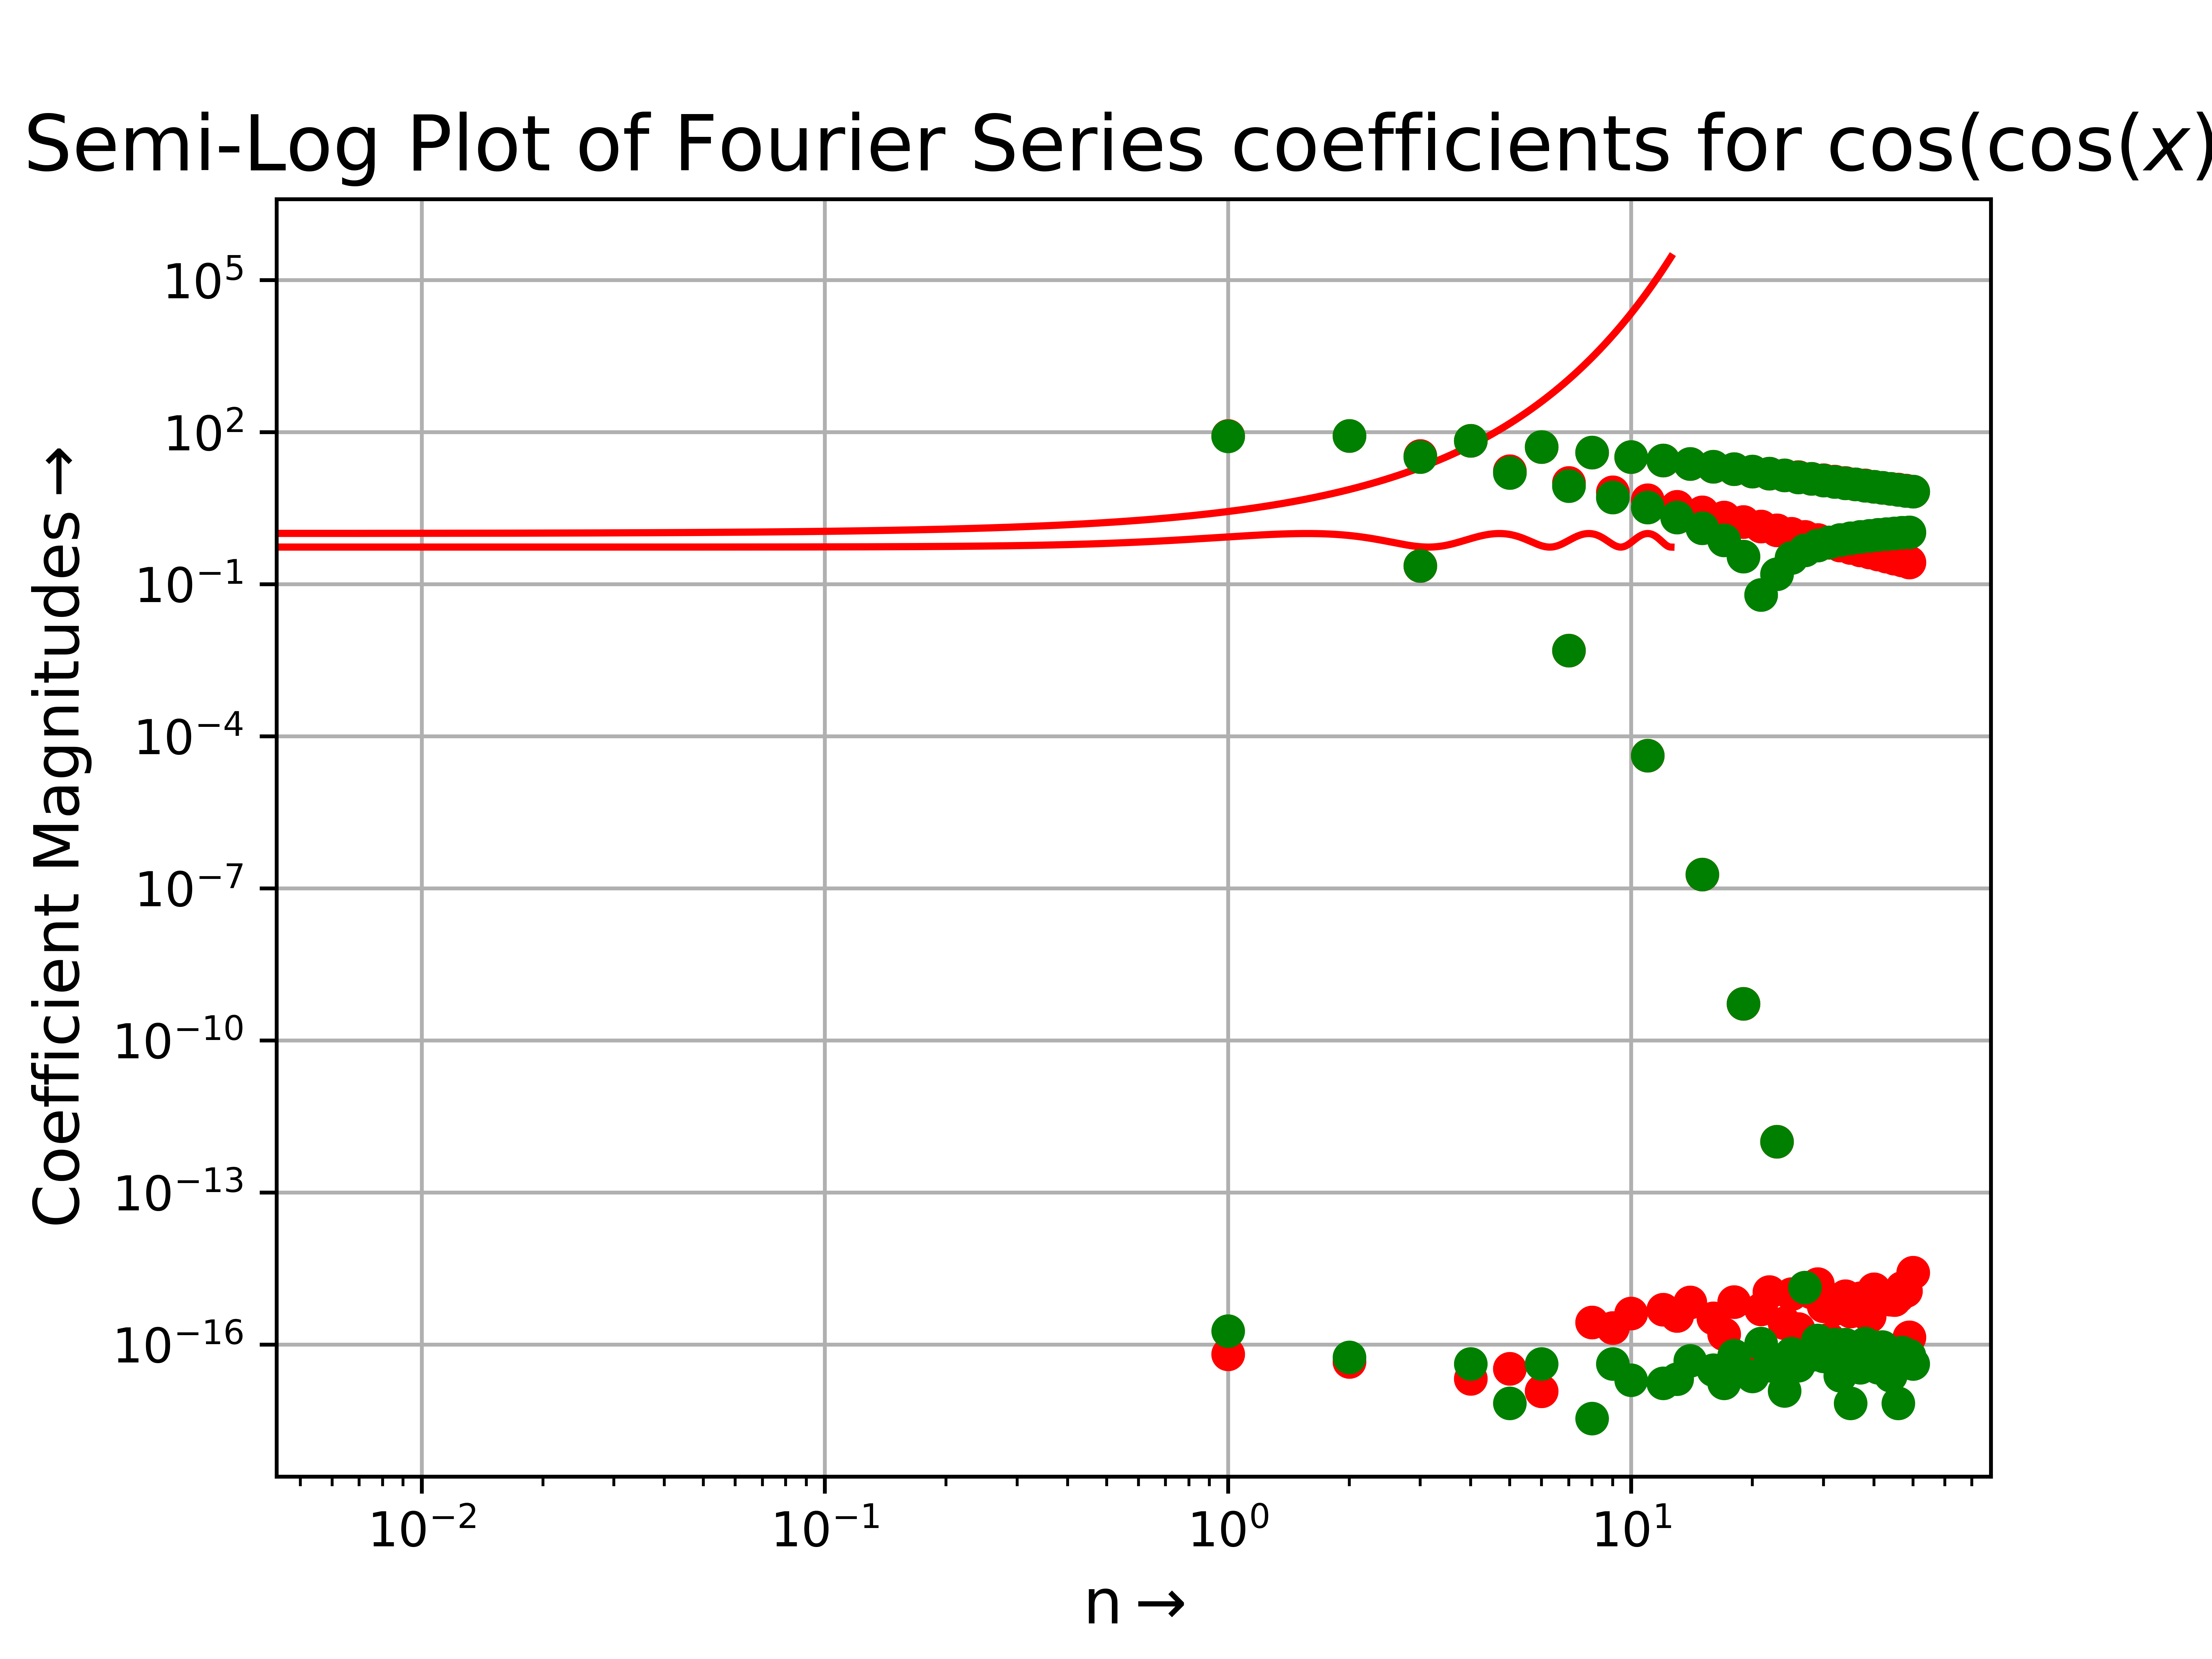
\includegraphics[scale=0.8]{images/Figure9.png}
\end{center}
\begin{center}
    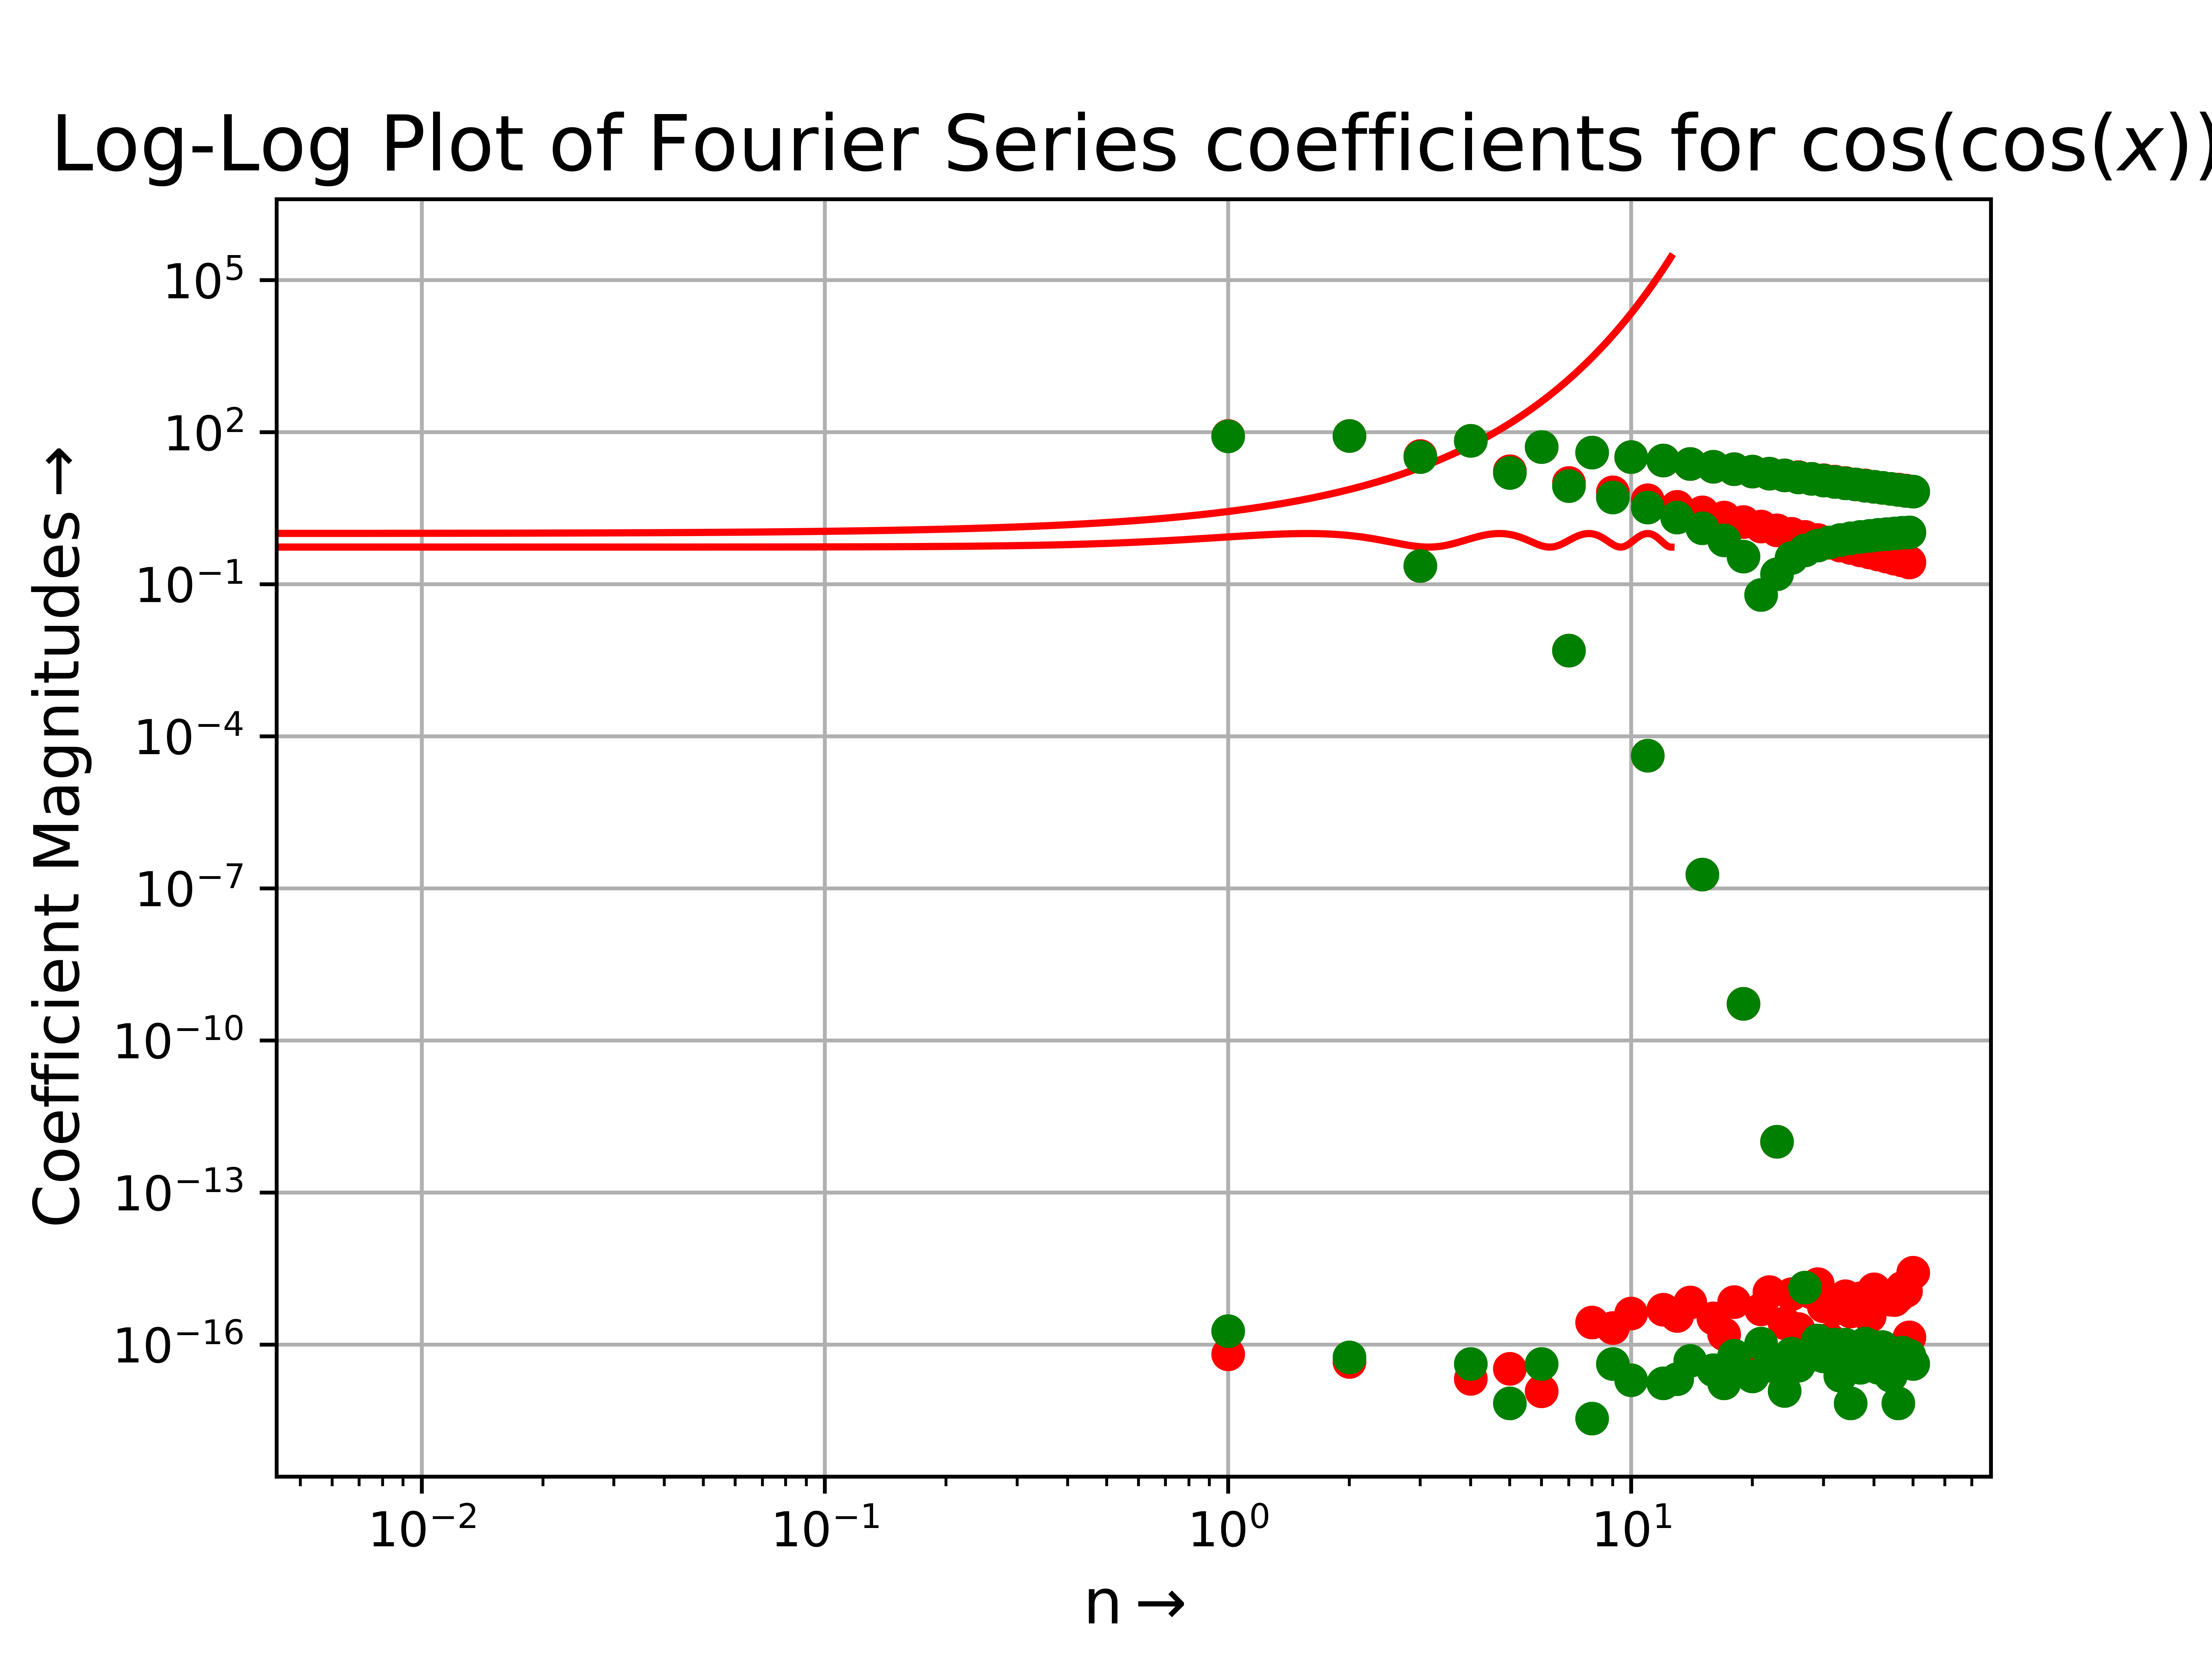
\includegraphics[scale=0.8]{images/Figure10.png}
\end{center}
\pagebreak

\section{Comparing between Direct Integration and Least Squares Approaches}

\subsection{Plots with both sets of Coefficients}

Now, we will plot both the sets of coefficients obtained from the Direct Integration as well as the Least Squares method together in one graph:

\bigskip
\bigskip

First, the $e^x$ function's coefficients:

\begin{lstlisting}
plt.semilogy(range(51),abs(expo_lstsq),'go',label='Least Squares Approach')
plt.semilogy(range(51),abs(expo_cfnts),'ro',label='Integration Approach')
plt.xlabel(r'n$\rightarrow$',fontsize=13)
plt.ylabel(r'Coefficient Magnitudes$\rightarrow$',fontsize=13)
plt.title('Semi-Log Plot of Fourier Series coefficients for $e^{x}$',fontsize=16)
plt.legend(loc='upper right')
plt.savefig("Figure11.png",dpi=1000)
plt.show()

plt.loglog(range(51),abs(expo_lstsq),'go',label='Least Squares Approach')
plt.loglog(range(51),abs(expo_cfnts),'ro',label='Integration Approach')
plt.xlabel(r'n$\rightarrow$',fontsize=13)
plt.ylabel(r'Coefficient Magnitudes$\rightarrow$',fontsize=13)
plt.title('Log-Log Plot of Fourier Series coefficients for $e^{x}$',fontsize=16)
plt.legend(loc='upper right')
plt.savefig("Figure12.png",dpi=1000)
plt.show()
\end{lstlisting}

\begin{center}
    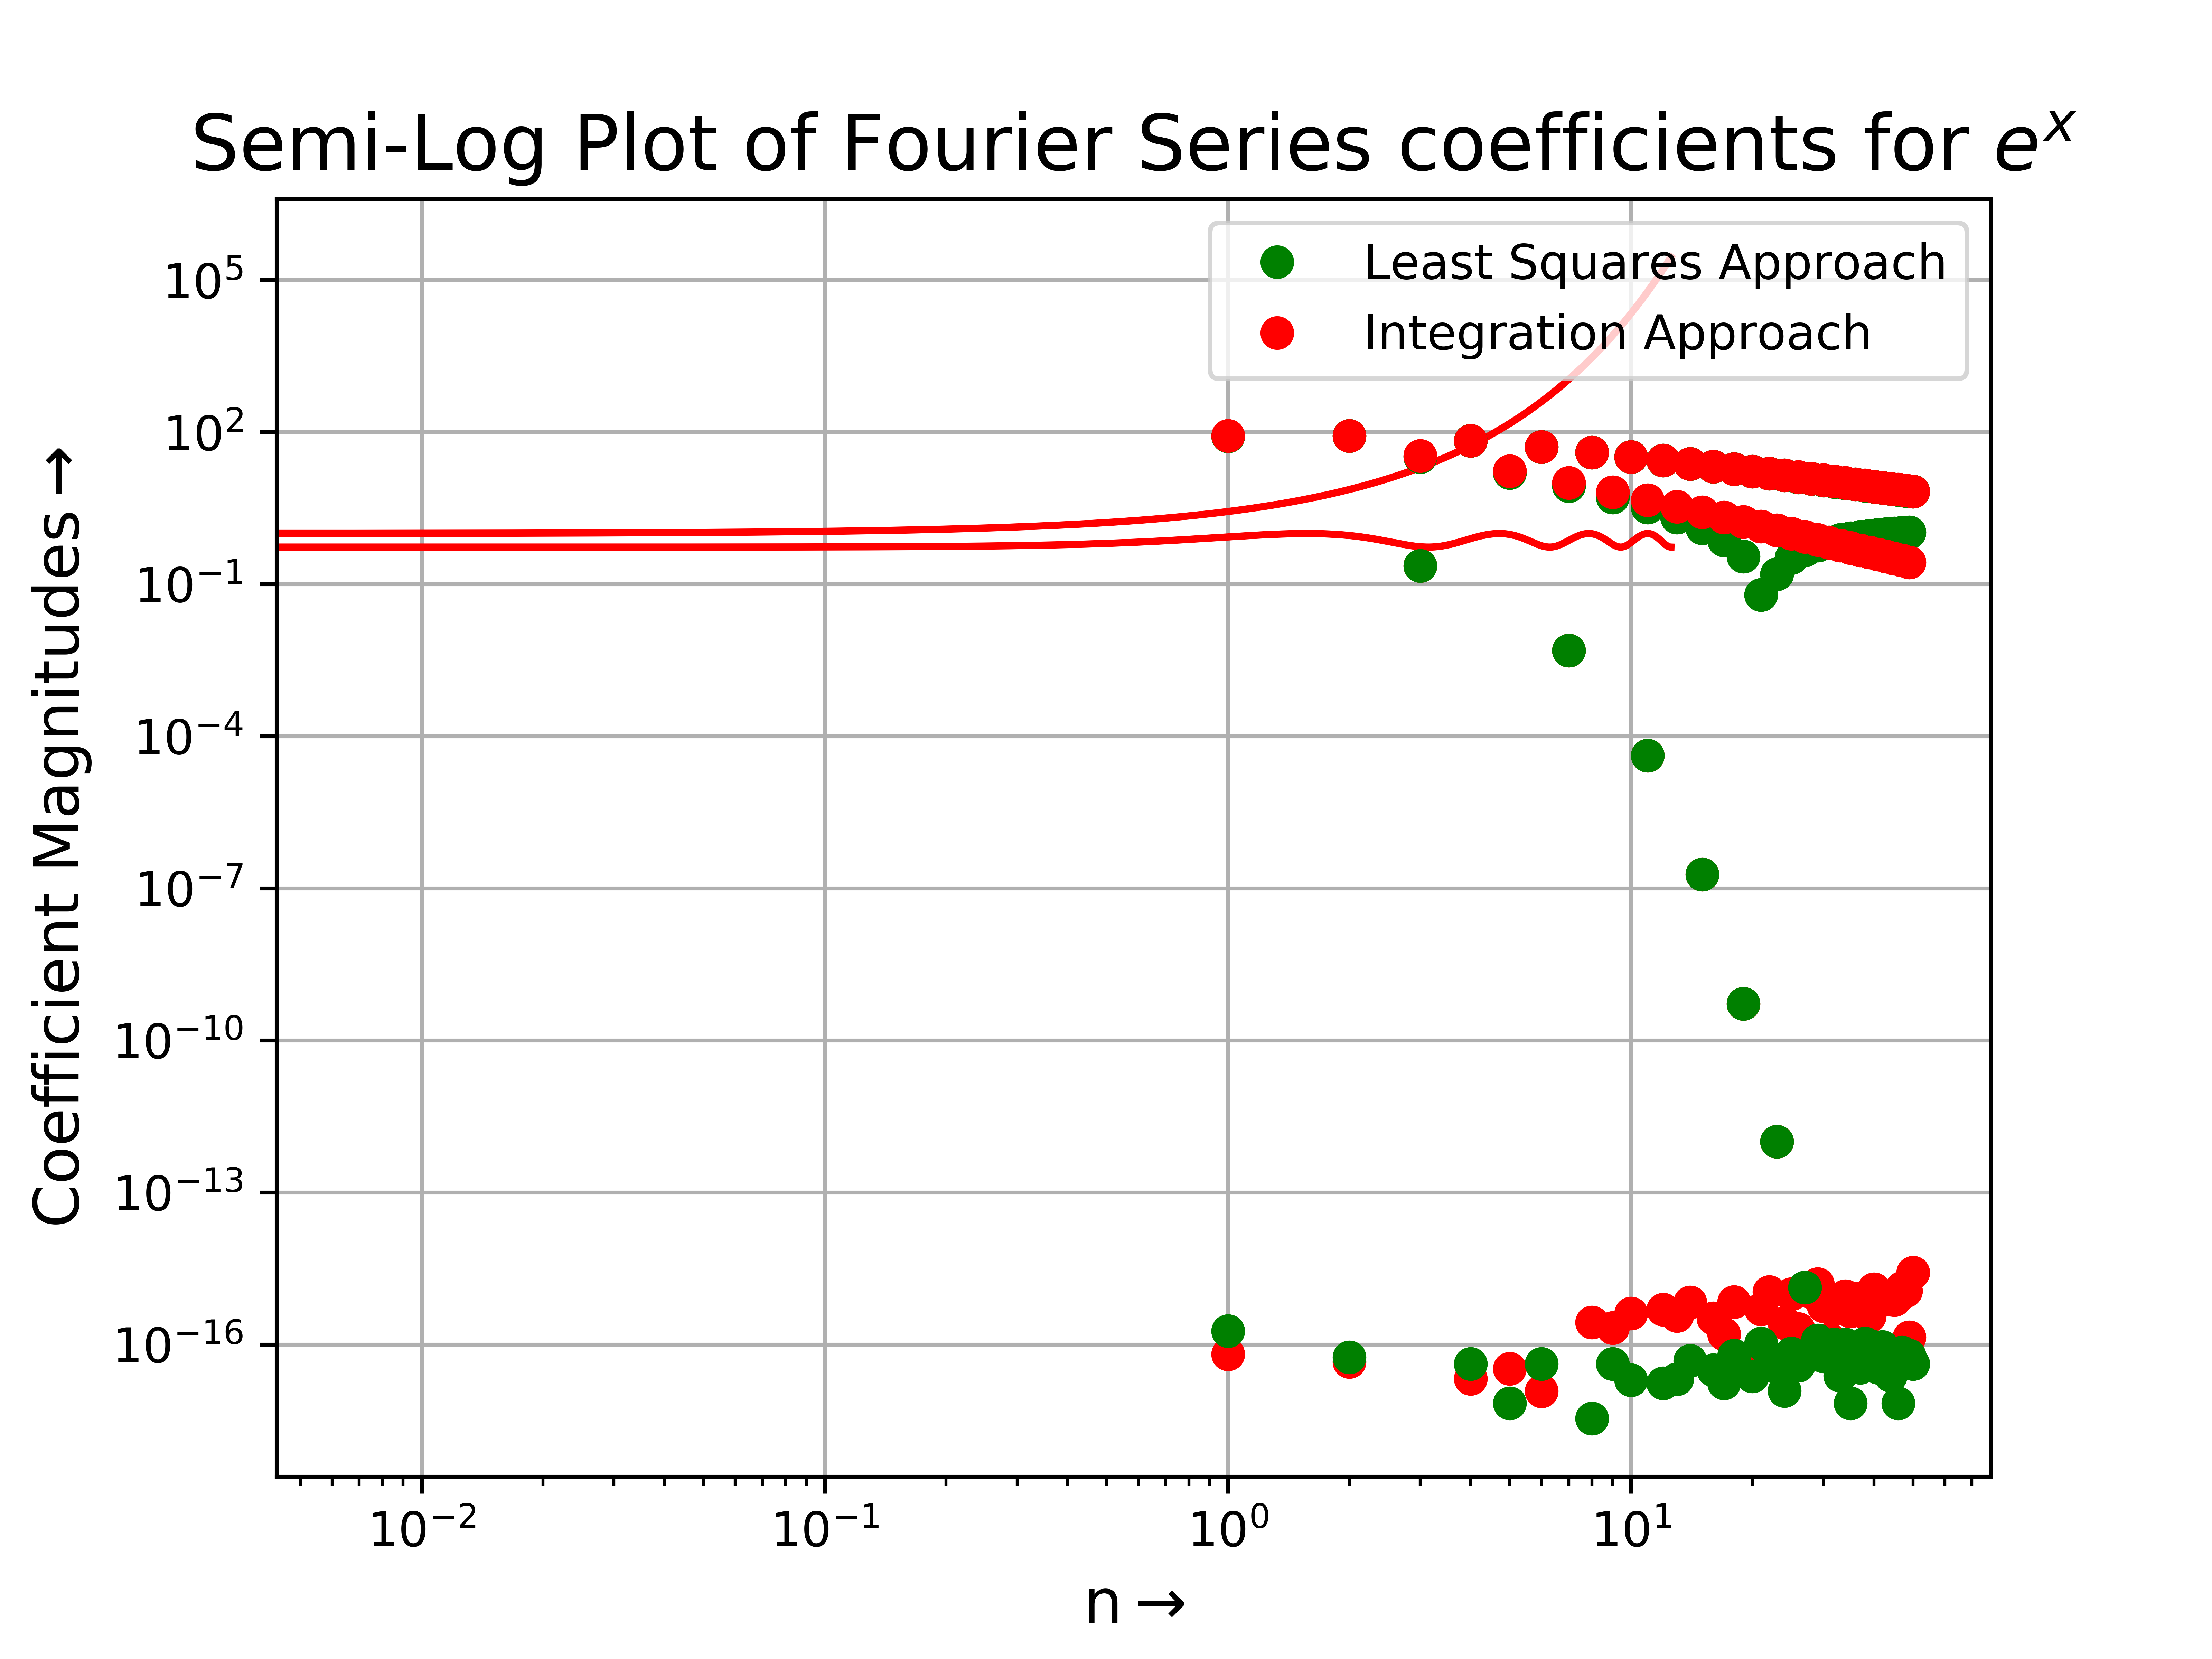
\includegraphics[scale=0.8]{images/Figure11.png}
\end{center}
\begin{center}
    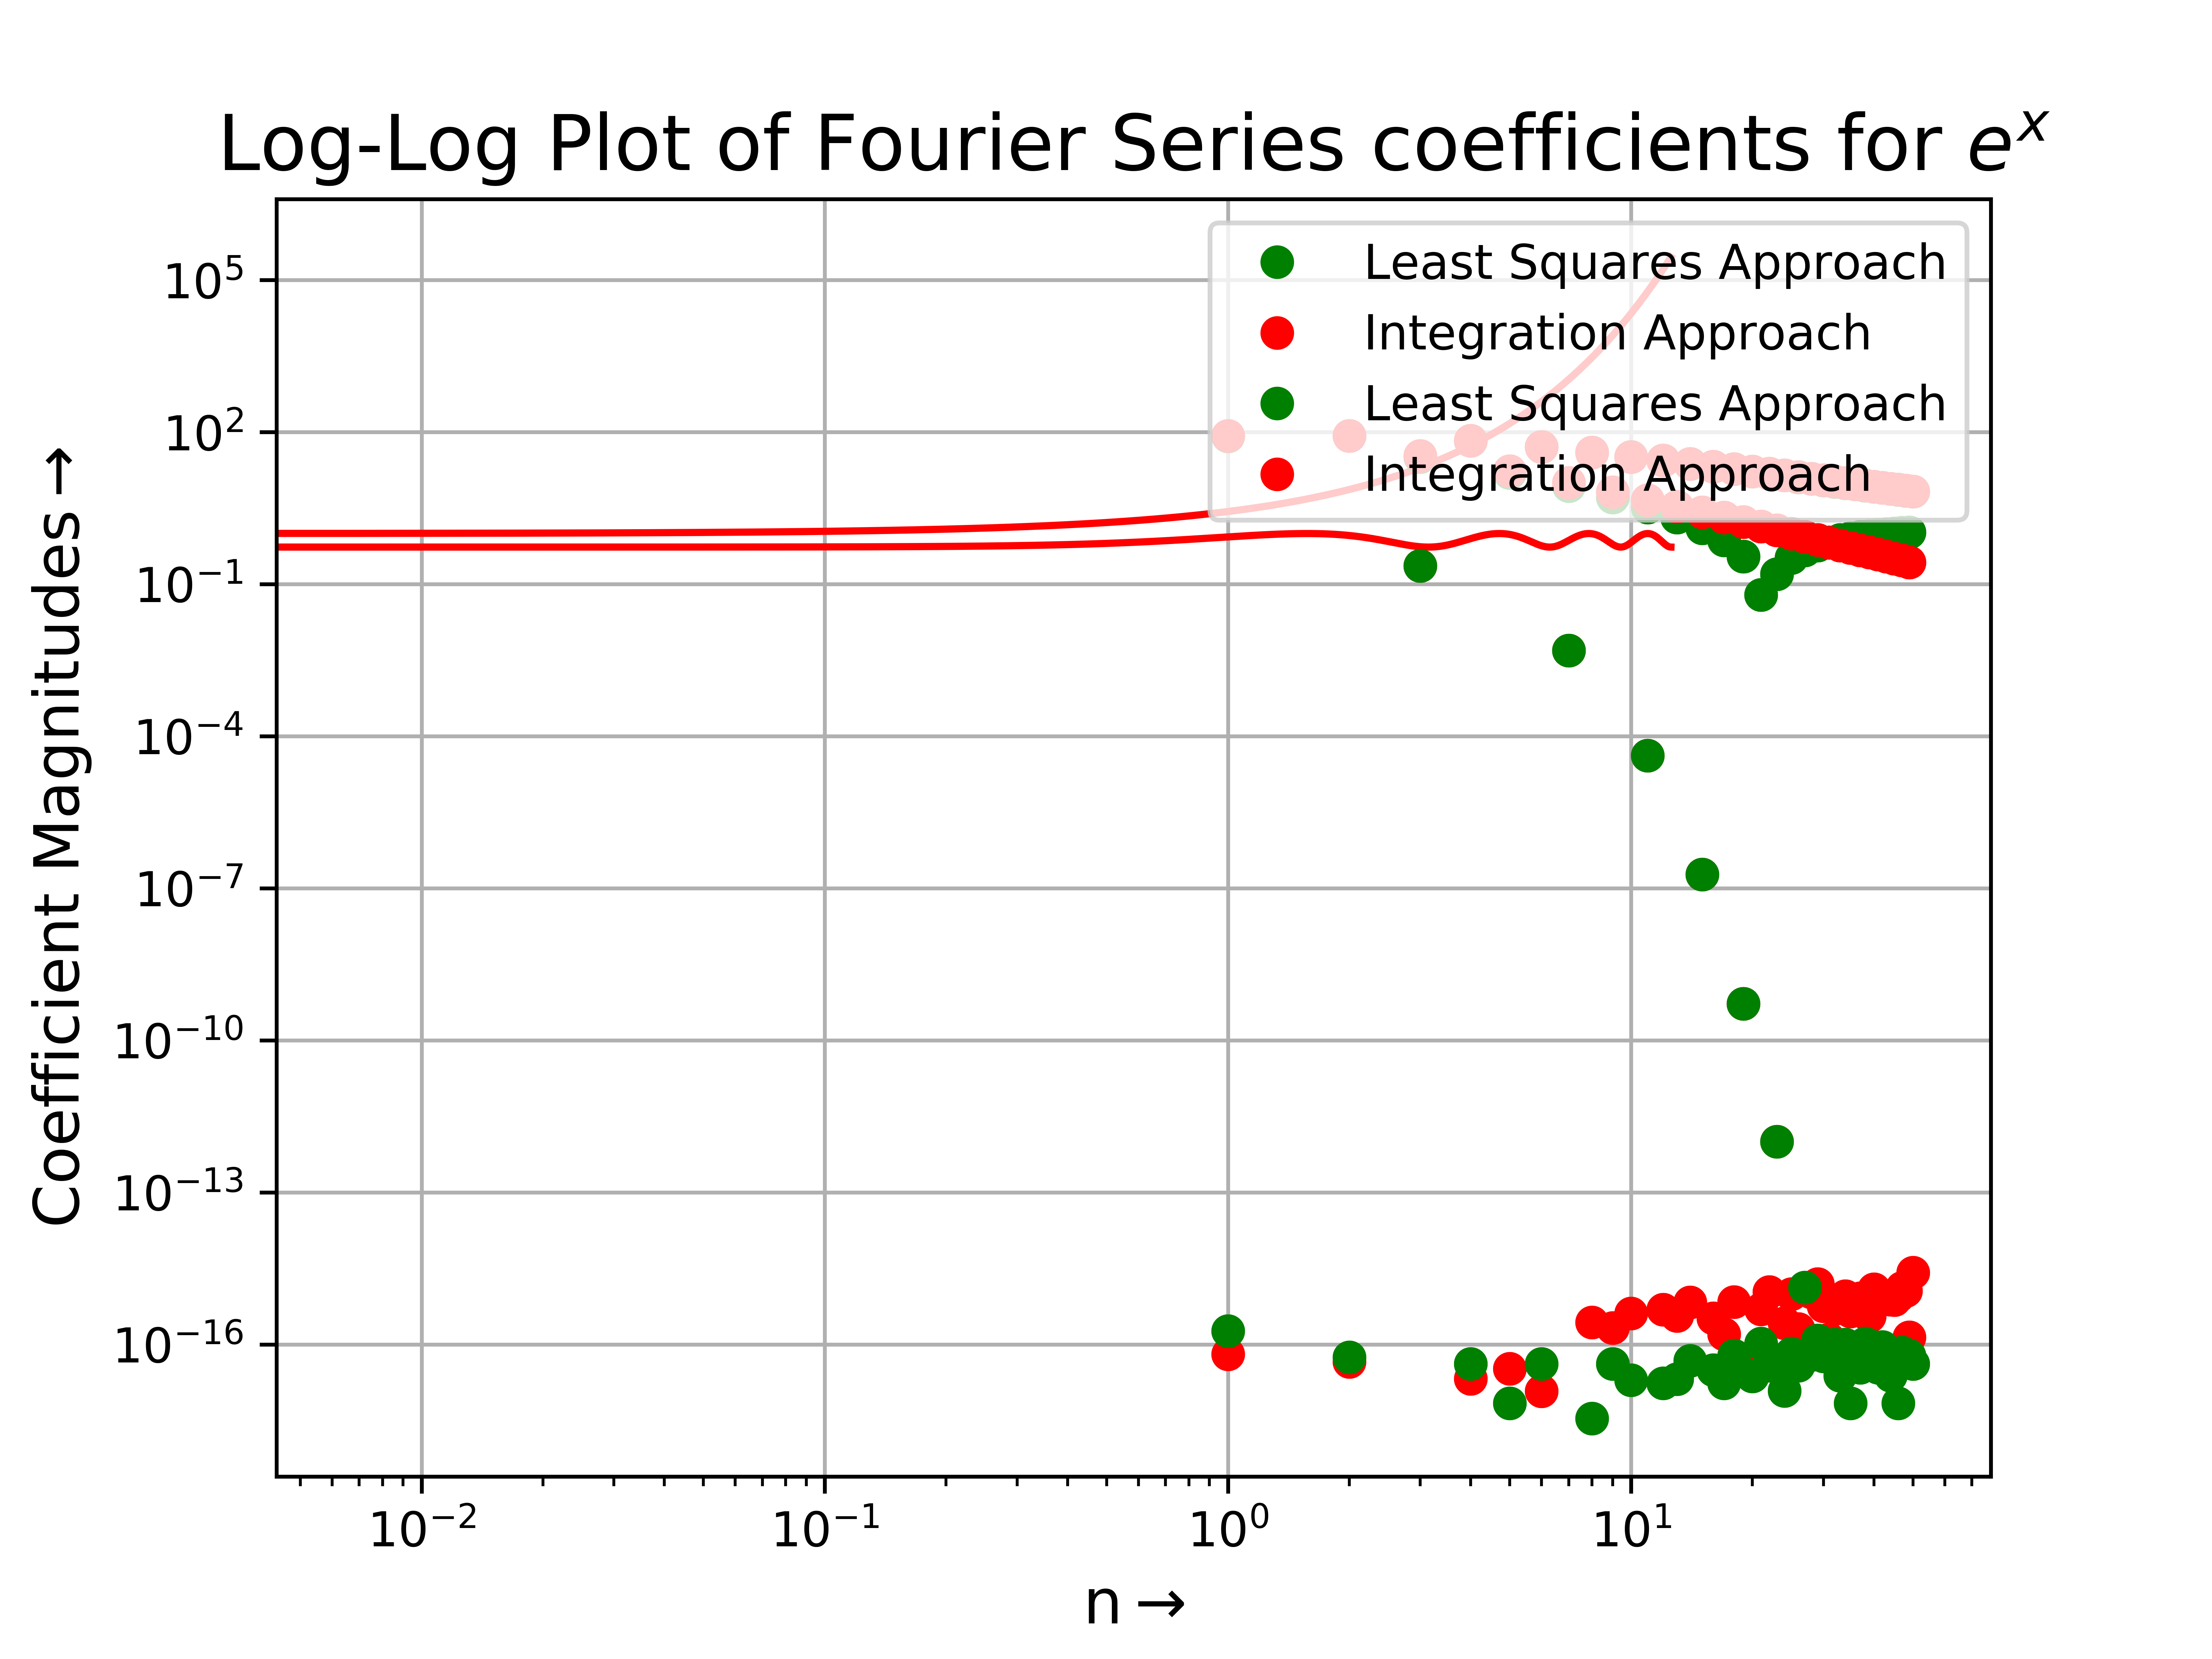
\includegraphics[scale=0.8]{images/Figure12.png}
\end{center}
\pagebreak

Next, the two sets of coefficients of the $\cos(\cos(x))$ function:

\begin{lstlisting}
plt.semilogy(range(51),abs(cc_lstsq),'go',label='Least Squares Approach')
plt.semilogy(range(51),abs(cc_cfnts),'ro',label='Integration Approach')
plt.xlabel(r'n$\rightarrow$',fontsize=13)
plt.ylabel(r'Coefficient Magnitudes$\rightarrow$',fontsize=13)
plt.title('Semi-Log Plot of Fourier Series coefficients for $\cos(\cos(x))$',fontsize=16)
plt.savefig("Figure13.png",dpi=1000)
plt.show()

plt.loglog(range(51),abs(cc_lstsq),'go',label='Least Squares Approach')
plt.loglog(range(51),abs(cc_cfnts),'ro',label='Integration Approach')
plt.xlabel(r'n$\rightarrow$',fontsize=13)
plt.ylabel(r'Coefficient Magnitudes$\rightarrow$',fontsize=13)
plt.title('Log-Log Plot of Fourier Series coefficients for $\cos(\cos(x))$',fontsize=16)
plt.savefig("Figure14.png",dpi=1000)
plt.show()
\end{lstlisting}

\begin{center}
    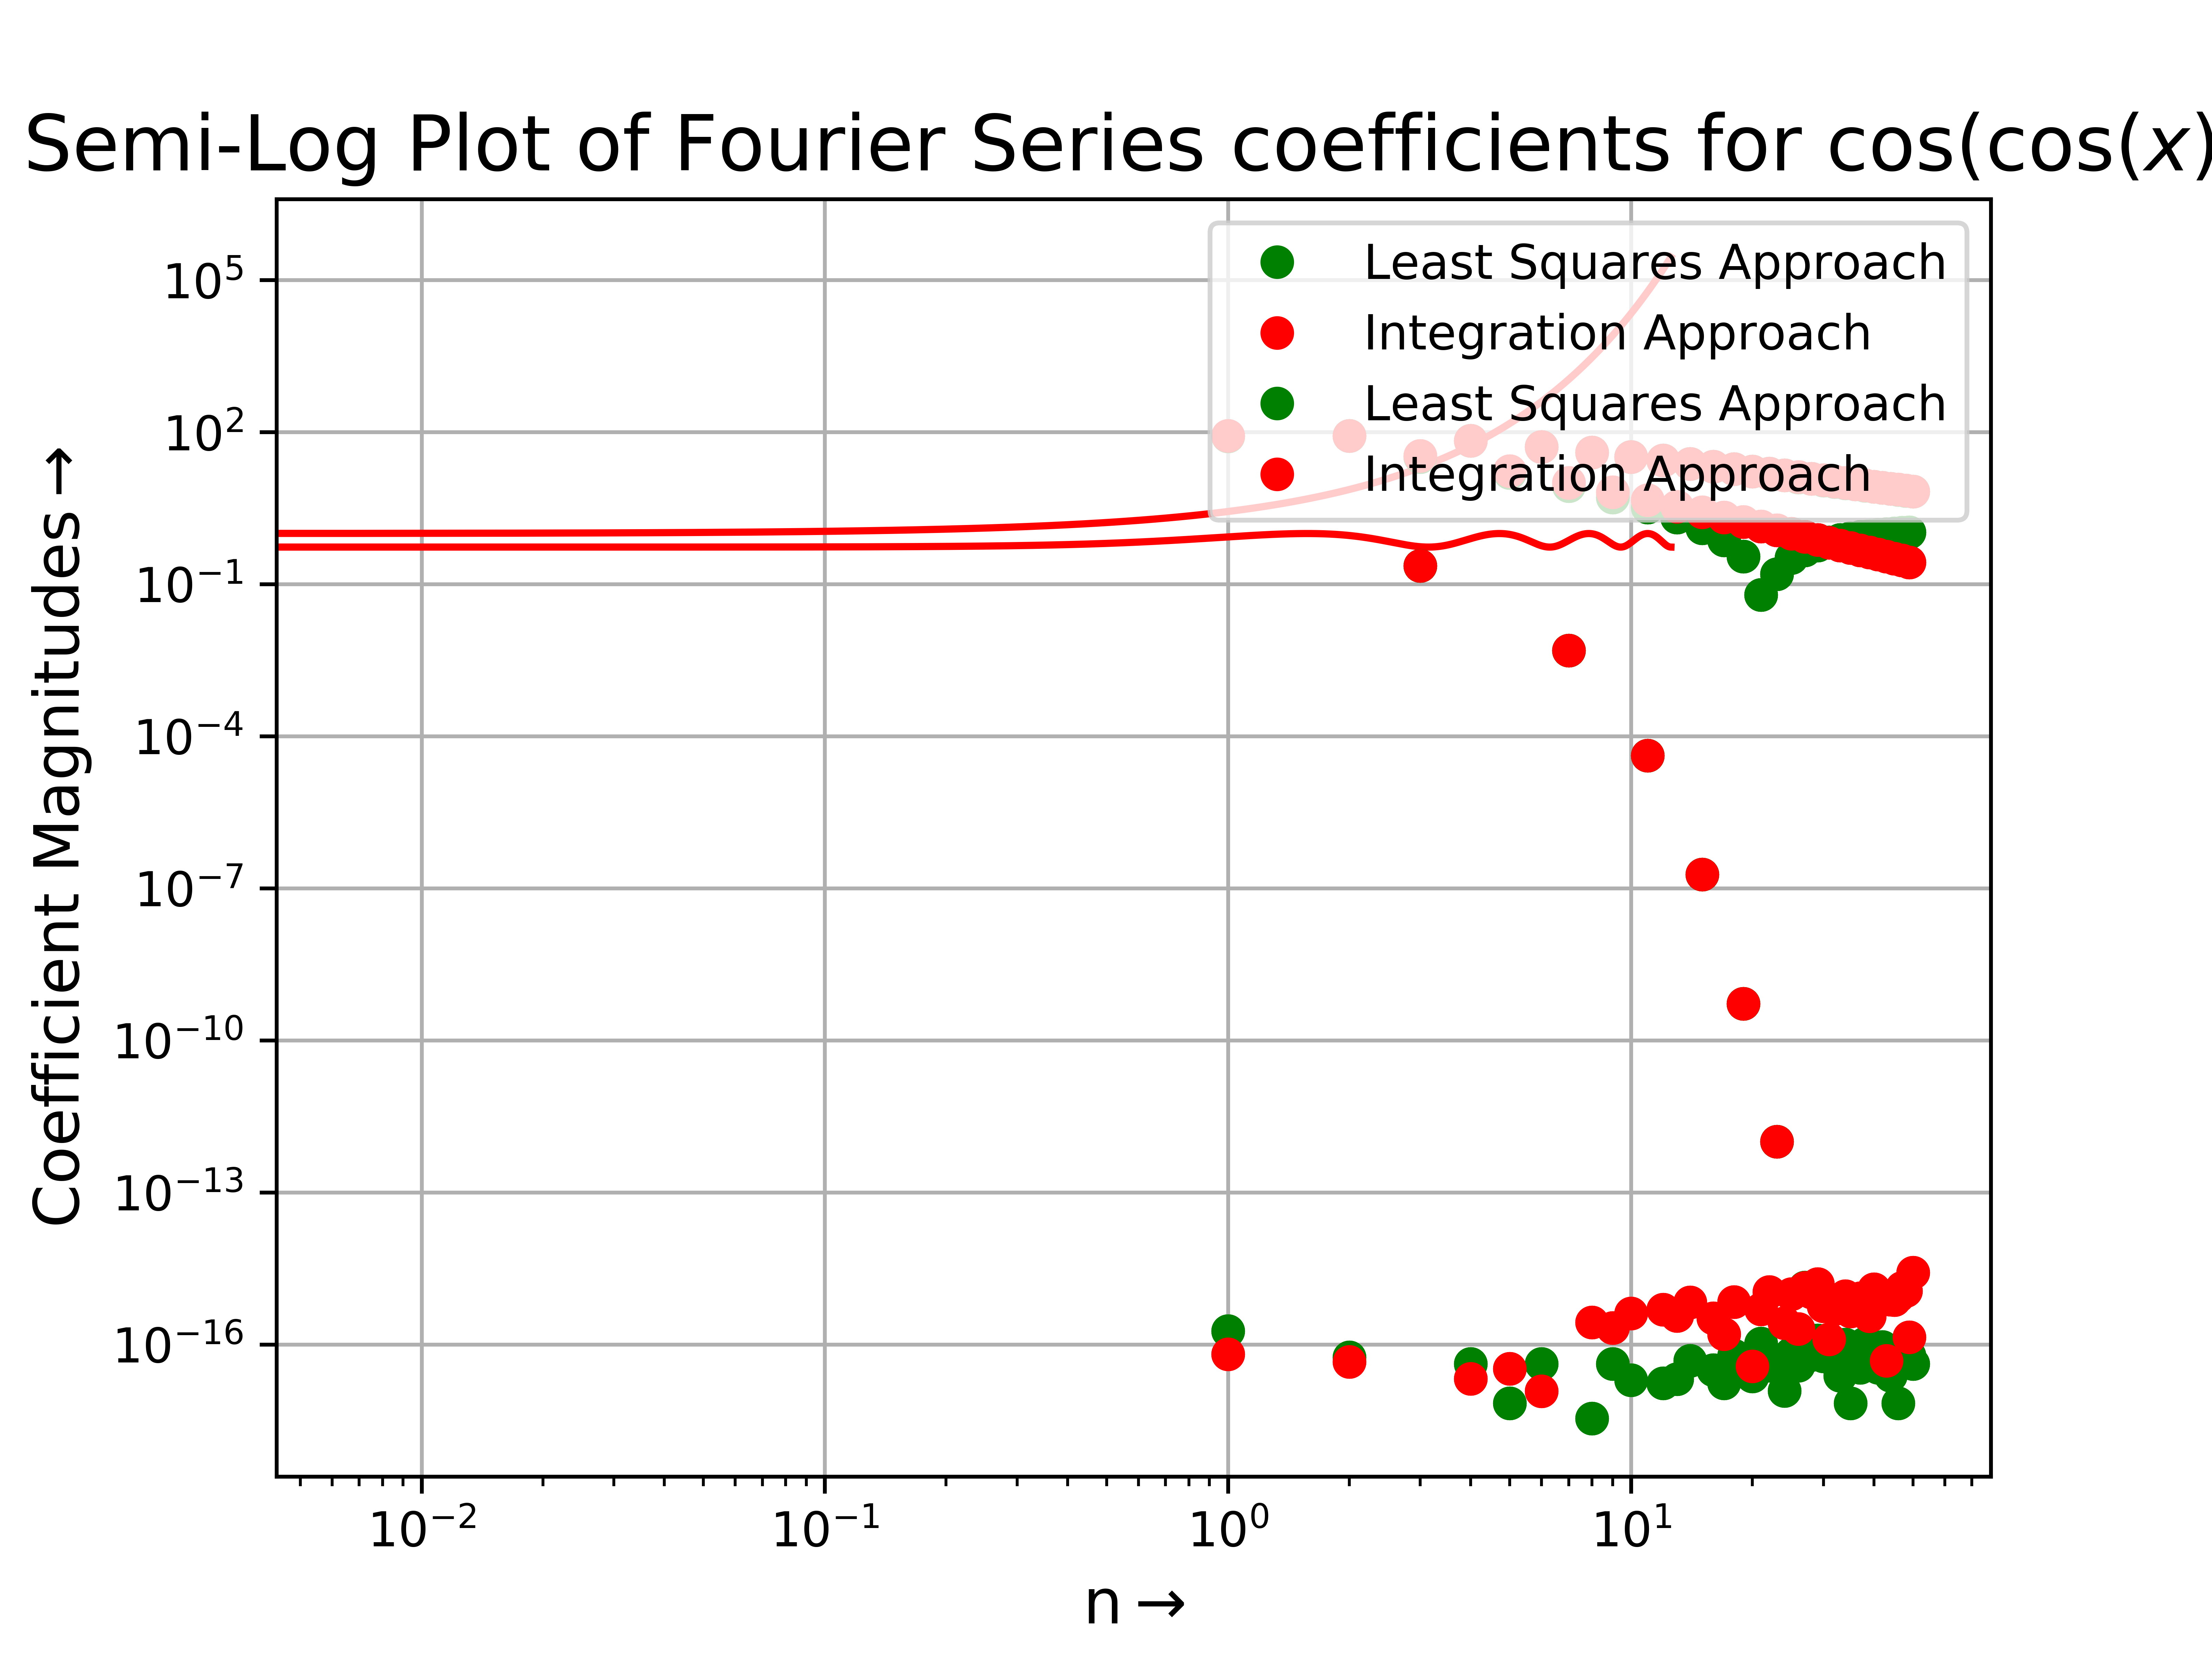
\includegraphics[scale=0.8]{images/Figure13.png}
\end{center}
\begin{center}
    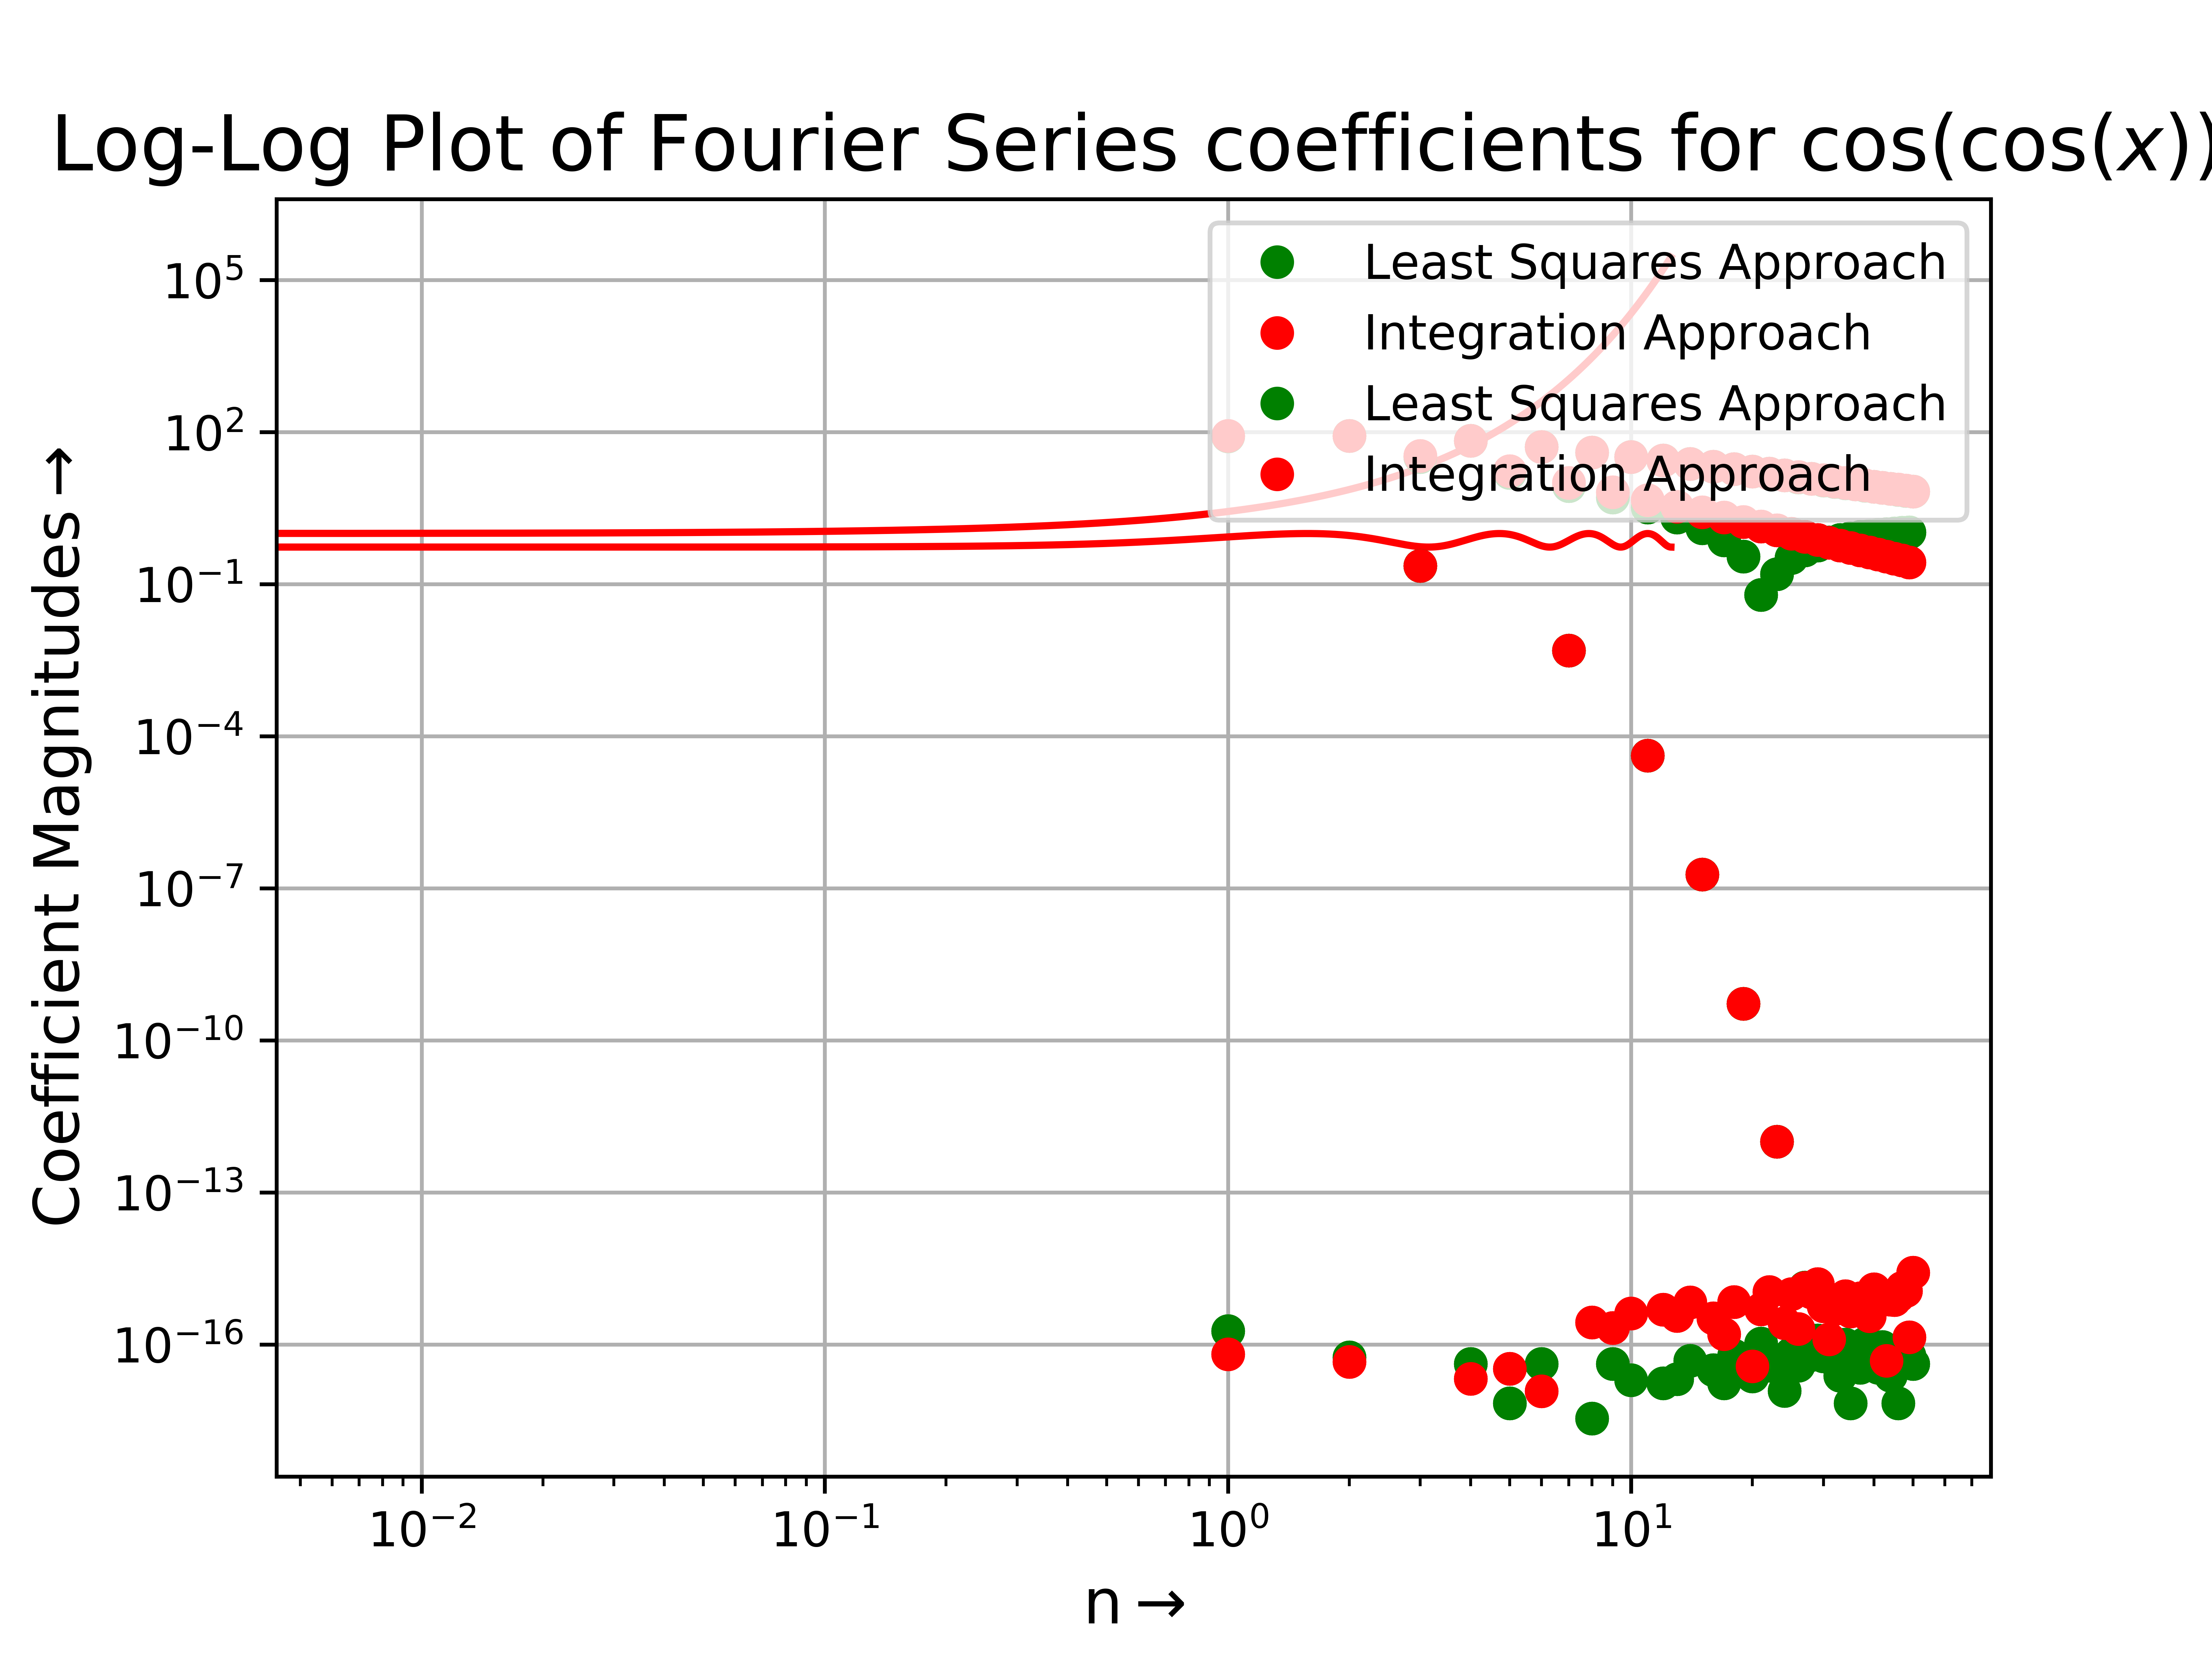
\includegraphics[scale=0.8]{images/Figure14.png}
\end{center}
\pagebreak

\subsection{Maximum Differences and Errors}

Using the following code, we find the maximum error between the two sets of coefficients we have found:

\begin{lstlisting}[language=Python]
dev_expo = abs(expo_lstsq-expo_cfnts)
dev_cc = abs(cc_lstsq-cc_cfnts)

maxdev_expo = np.max(dev_expo)
maxdev_cc = np.max(dev_cc)

print(maxdev_expo)
print(maxdev_cc)
\end{lstlisting}

The output was:

\begin{lstlisting}
1.3327308703354106
2.646921459797403e-15
\end{lstlisting}

This clearly shows that the exponential function is quite a bit different, while the $\cos(\cos(x))$ function is very close to the actual function.

\subsection{Comparing Times taken}

\begin{lstlisting}[language=Python]
print(delTime1)
print(delTime2)
print(delTime3)
print(delTime4)
\end{lstlisting}

The output was:

\begin{lstlisting}[language=Python]
0.0380091667175293
0.020006179809570312
0.0026311874389648438
0.0010001659393310547
\end{lstlisting}

\begin{lstlisting}
1.3327308703354106
2.646921459797403e-15
\end{lstlisting}


\subsection{Plots of Actual function vs Fourier Approximation found using Least Squares}

Finally, we plot the Actual Functions vs their Fourier Approximations that we found using Least Squares

First, for the Exponential:

\begin{lstlisting}[language=Python]
expo_approx = A@expo_lstsq

plt.semilogy(x,expo_approx,'go',label='Approximation')
plt.semilogy(x,expo(x),'-r',label='Actual value')
plt.grid(True)
plt.xlabel(r'n$\rightarrow$',fontsize=13)
plt.ylabel(r'$f(x)\rightarrow$',fontsize=13)
plt.title('Plot of $e^{x}$ vs Fourier series approximation to 51 terms',fontsize=16)
plt.legend(loc='upper left')
plt.savefig('Figure15.png',dpi=1000)
plt.show()

\end{lstlisting}

\begin{center}
    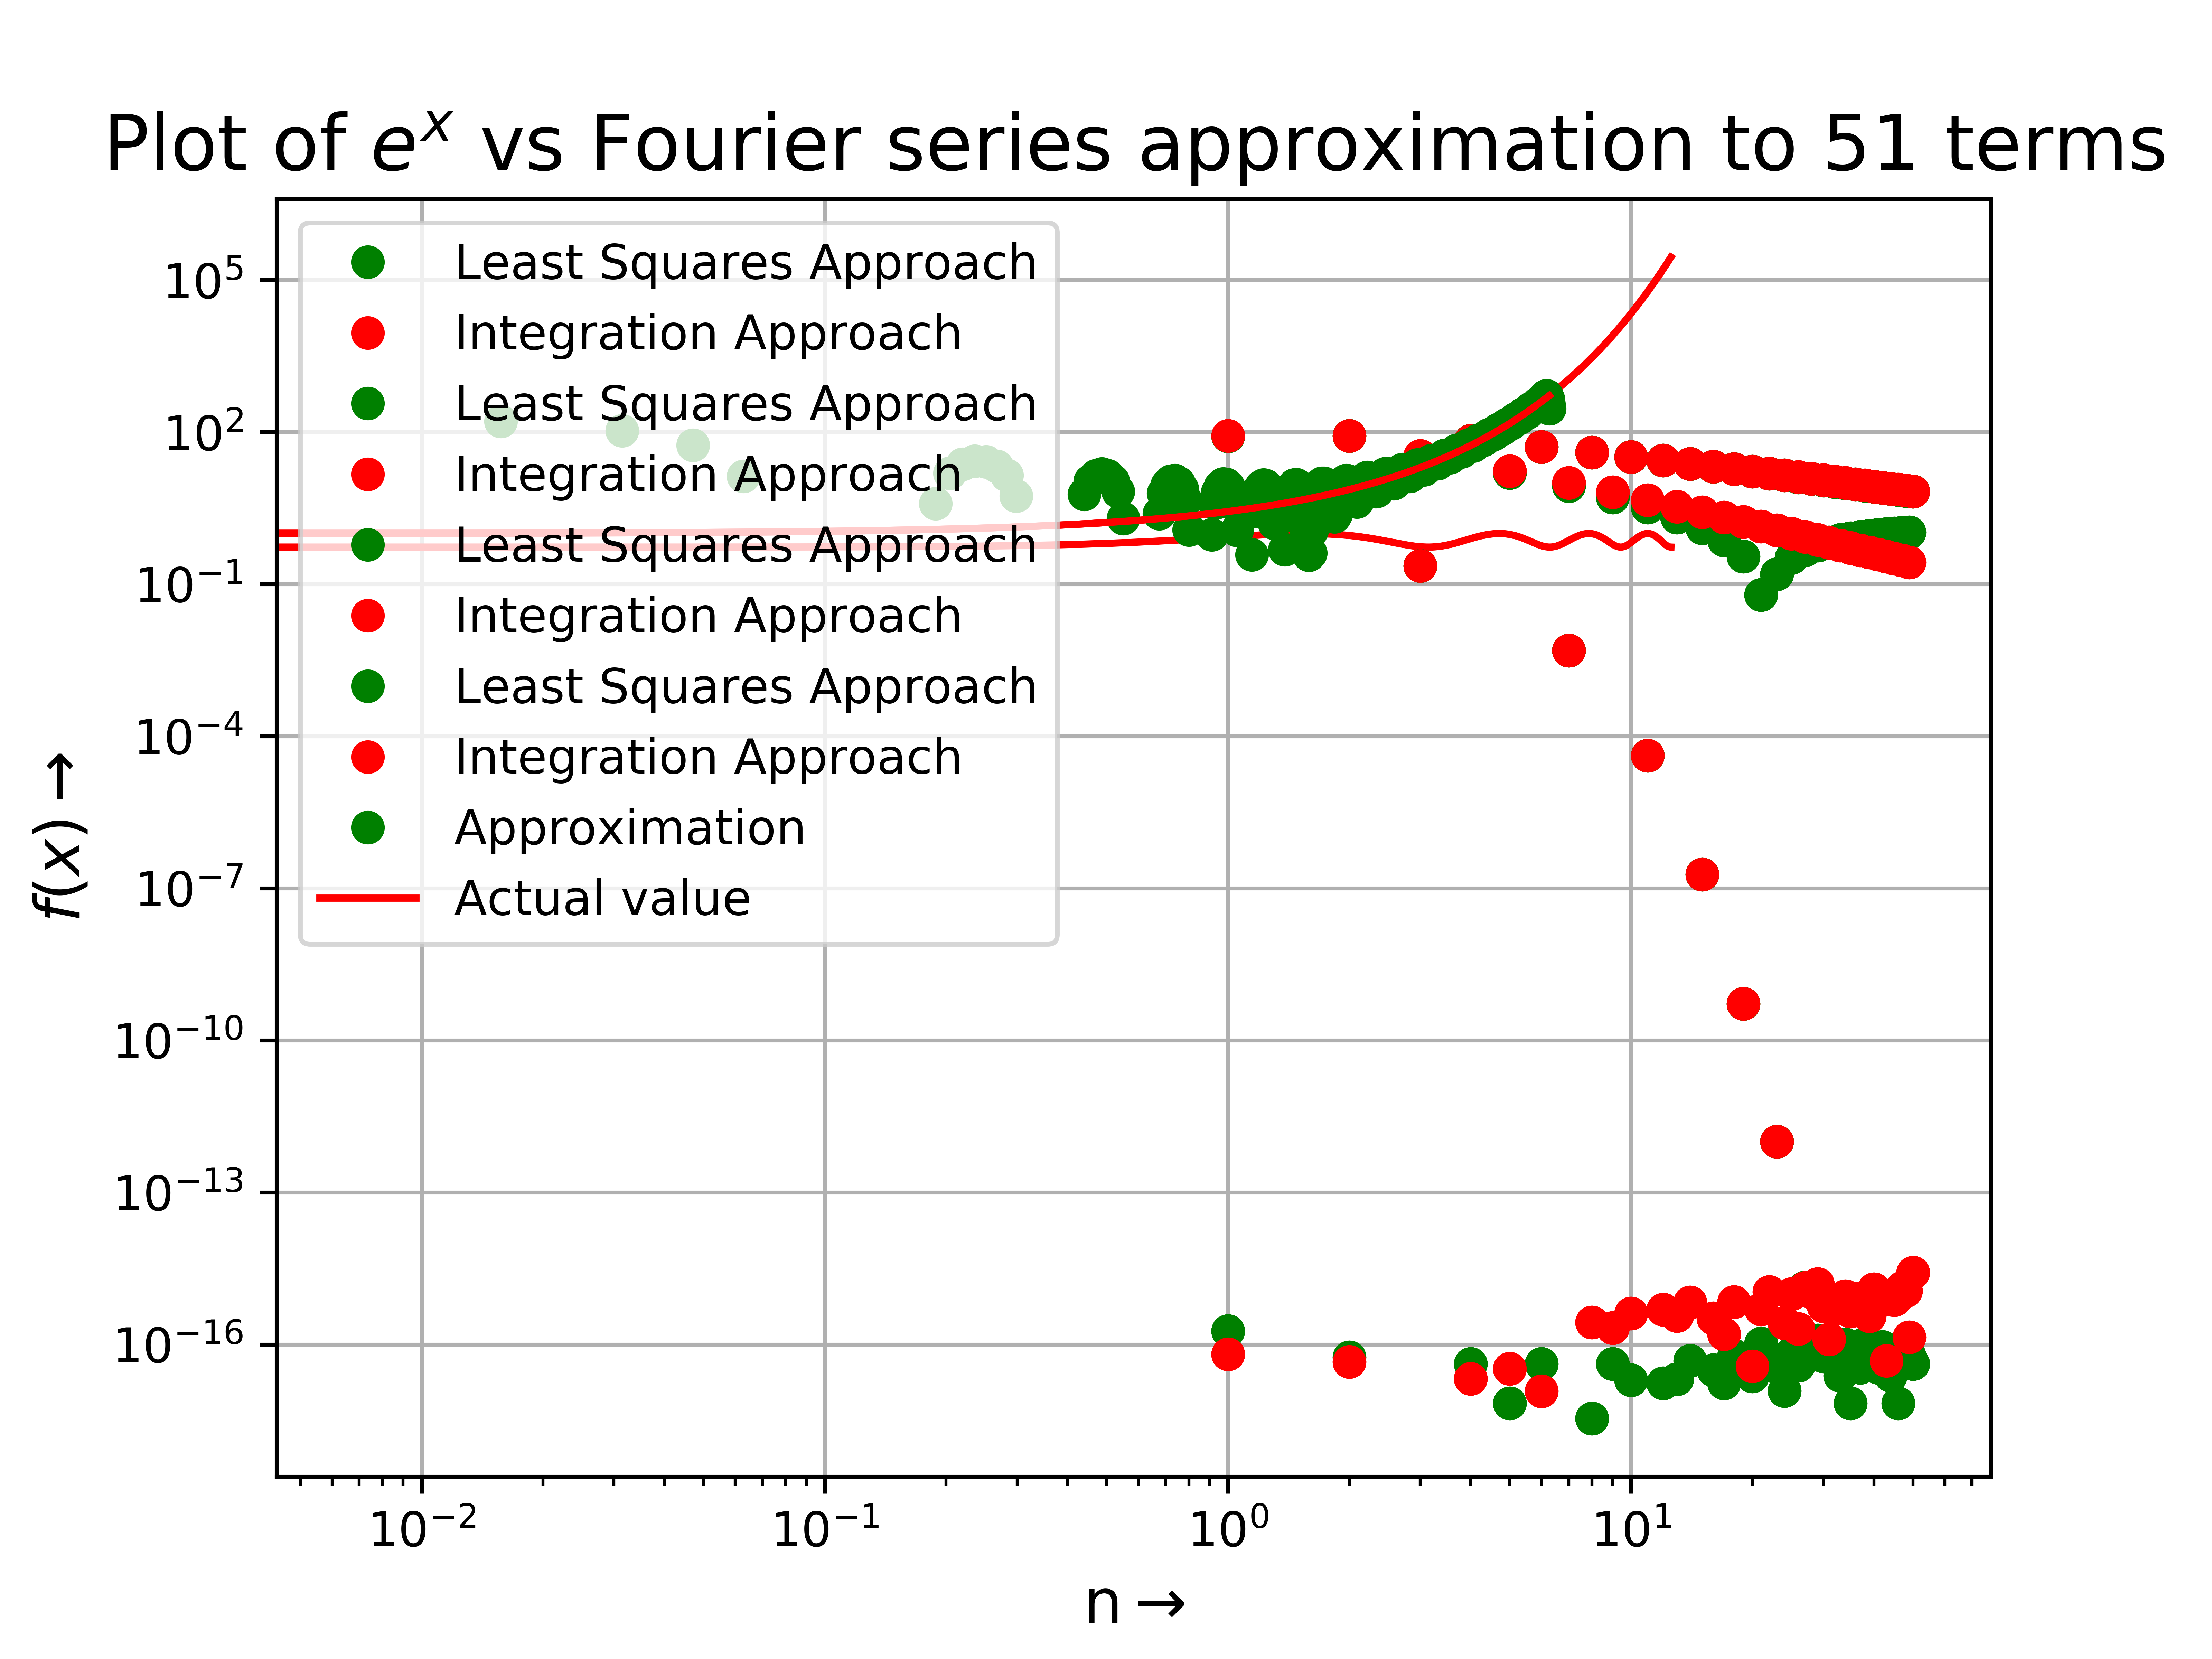
\includegraphics[scale=0.8]{images/Figure15.png}
\end{center}

The exponential is very different from the actual function due to the fact that it is not periodic and has very high frequency components involved in it due to its large values. Hence, it is very difficult to approximate it using a Fourier Series.

\pagebreak

Next, the $\cos(\cos(x))$ function:

\begin{lstlisting}[language=Python]
cc_approx = A@cc_lstsq
plt.plot(x,cc_approx,'go',label='Approximation')
plt.plot(x,cc(x),'-r',label='Actual value')
plt.grid(True)
plt.xlabel(r'n$\rightarrow$',fontsize=13)
plt.ylabel(r'$f(x)\rightarrow$',fontsize=13)
plt.title('Plot of $\cos(\cos(x))$ vs Fourier series approximation to 51 terms',fontsize=16)
plt.legend(loc='upper left')
plt.savefig('Figure16.png',dpi=1000)
plt.show()
\end{lstlisting}

\begin{center}
    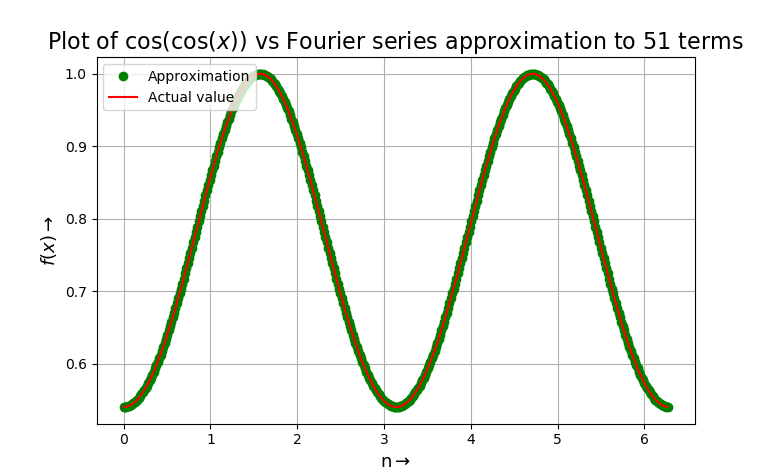
\includegraphics[scale=0.8]{images/Figure17.png}
\end{center}

Clearly, this seems to line up pretty accurately, since $\cos(\cos(x))$ is a periodic function and hence has a converging Fourier Series approximation.

\pagebreak
\section{Overall Conclusions for Least Squares Method vs Direct Integration}
\begin{enumerate}
    \item In terms of time, the Direct Integration method took 14 times the time taken by Least Squares for the $e^x$ function, and 20 times the time taken for the $\cos(\cos(x))$ function. Thus, the Least Squares method is better in terms of speed, but this speed effect only becomes apparent for larger values of n.
    \item The Direct Integration method is clearly established to be the more accurate method, although, the error in the $e^x$ function in the Least Squares method stems from the fact that the exponential function has a large number of high frequencies involved, and is not periodic.
    \item As a whole, both the methods are equally accurate for approximating periodic functions with fewer coefficients, but Least Squares is computationally much less expensive.
\end{enumerate}


\end{document}